% Need to discuss how we put data, the background estimate, and the signal model together
%     and make a claim as to the compatibility of the hypothesis with the data.
% Largely, this means I need to finally understand how pyhf actually works and what the hell the limit framework is doing.
\chapter{Results} \label{chapter:results}

%
%
%
%    I'm not sure I actually have to explain Baye's theorem here...
%    it doesn't appear to be obviously used, or if it is, we're implicitly using the "Uniform" Prior
%    Ask Steve
%
%    L gives probability of seeing the data we have, based on the given model.
%    We need the probability that the given model is the one responsible for the data we see.
%    i.e. we have P(data|model), but we need P(model|data)
%
%    To do this, we need Baye's rule, which comes from the basic 'anding' of probabilities:
%    P(a \& b) = P(a)*P(b|a) , or P(a \& b) = P(b)*P(a|b) . Thus
%    P(a)*P(b|a) = P(b)*P(a|b) 
%    P(b|a) = P(a|b) P(b) / P(a)
%    So we need P(model|data) = P(data|model) * P(model) / P(data)
%
%    For our data we have to use the extended L, which accounts for poisson stats.
%    Basic test is to test mu*S+B for what value of mu is compatible with data
%
%        
%
%
%Statistics is a powerful tool in science,
%    but one which can be very misleading if not used carefully.
%%The oft-used quote comparing lies and statistics exists for a reason;
%%    both can lead to incorrect scientific conclusions.
%%But whereas a lie can be caught by a simple slip of the tongue,
%%    it can take scientists years to discover a slight (intentional or not) mishandling of statistics.
%Unfortunately, the use of statistical methods is not optional.

%To begin, let me propose a much simpler experiment than the one described in this analysis.
%I have a coin, which I suspect may be biased to one side.
%How can I test this?
%A fair coin has a 50/50 chance of landing on either side.
%This means that, were I to flip the coin a large number of times,
%    I would expect a roughly equal number of heads and tails.
%Significant deviation from this ratio (e.g.\ 3 million heads to 1 million tails)
%    would indicate an obvious bias in the coin.
%The conclusion becomes far less obvious however, if the coin is flipped only a few times.
%Even if every flip comes up as heads, no meaningful conclusion can be made if the coin was only flipped e.g.\ four times.
%The crucial questions raised here, which statistical methods are able to address,
%    are how much data is needed to make a decisive statement about a hypothesis,
%    and what kind of statements can be made in lieu of that data.

%The first step to testing a hypothesis,
%    is to know precisely how \textit{likely} any particular outcome is based on that hypothesis.
%The hypothesis for the coin flip is that the probability $p$ of any given flip being heads is 50\%.
%For an experiment consisting of a number of flips $N$,
%    the overall probability of seeing an amount of heads $n$ is given by the binomial distribution:
%\begin{equation}
%    P(n|p) = \tinymatrix{N\\n} p^n (1-p)^{N-n}
%\end{equation}
%Where $P(n|p)$ is read as ``the probability of seeing $n$ heads \textit{given} their probability $p$.''
%With this, 
%
%basic binomial distribution (coin flip) allows obvious p-test. 
%Using a concrete toy example with numbers,
%Show a binomial PDF distro for N flips, and where on that distro the "data" lies
%Show a C-PDF, and again where the data is,
%    and explain that the "unlikeliness" can be used as a test metric, called a "p-value"
%Show of whether or not theory is compatible with data.


% NOTE: From here on, try to keep the p-value concept,
%   as well as the PDF and C-PDF, as a central focus.
% It's easy to conceptualize what a p-value is,
% so you should keep returning to it in order to retain 
% a concrete basis for all the weird math you're about to do
\section{Statistical Mathematics}

    I have thus far established how the analysis has collected its data,
        how it has estimated the amount of background present in that data,
        and how it has modeled the hypothesis for the HH process to be tested with that data.
    With these assembled, the final step is to arrange them together in order to make a definitive statement
        as to the validity or incompatibility of the hypothesis with the provided data.
    More plainly, the questions for this chapter are:
        was the di-Higgs process detected in the data,
        and what were the values of the $\kappa$ couplings involved in its production?
    To answer these questions, I must turn to the field of statistical analysis.
    In this chapter, I want to explain why statistics is required for this analysis,
        discuss the specific statistical techniques this analysis uses,
        and conclude with what those techniques reveal in light of the data presented.

    % Introduce poisson statistics with single counting variable and only signal w/ toy example.
    % Discuss difference between coin toss and radioactivity.
    % i.e. that with a coin toss, the number to tosses is entirely determined by me, and is thus fixed.
    % For decay and such, the number of events is completely random, and what is fixed is how much time (luminosity)
    %     the experiment is given.
    Like most particle physics processes [all?], the $VBF \to HH \to 4b$ process is poisonian in nature.
    The number $n$ of di-Higgs process that are observed in ATLAS can then be modeled with a Poisson distribution\cite{cranmer2015practical}:
    \begin{equation}
        P(n|\nu) = \frac{ \nu^n e^{-\nu} }{n!}
    \end{equation}
    Where $\nu$ is the expected event yield for the process.
    The compatibility of a hypothesis with data can be established by use of a ``p-value test.''
    As an example, take the case of a simple alpha emitter,
        which I hypothesize emits radiation at a rate of once per minute.
    After one hour, I would expect on average 60 events.
    Running the experiment, I find that 68 events were detected.
    Plotting the Poisson distribution for $P(n|60)$ (Fig. \ref{fig:poisson_toy_sig:pdf}),
        I can see how likely an observation of 68 events is.
    \begin{figure}
        \centering
        \begin{subfigure}{0.48\textwidth} 
            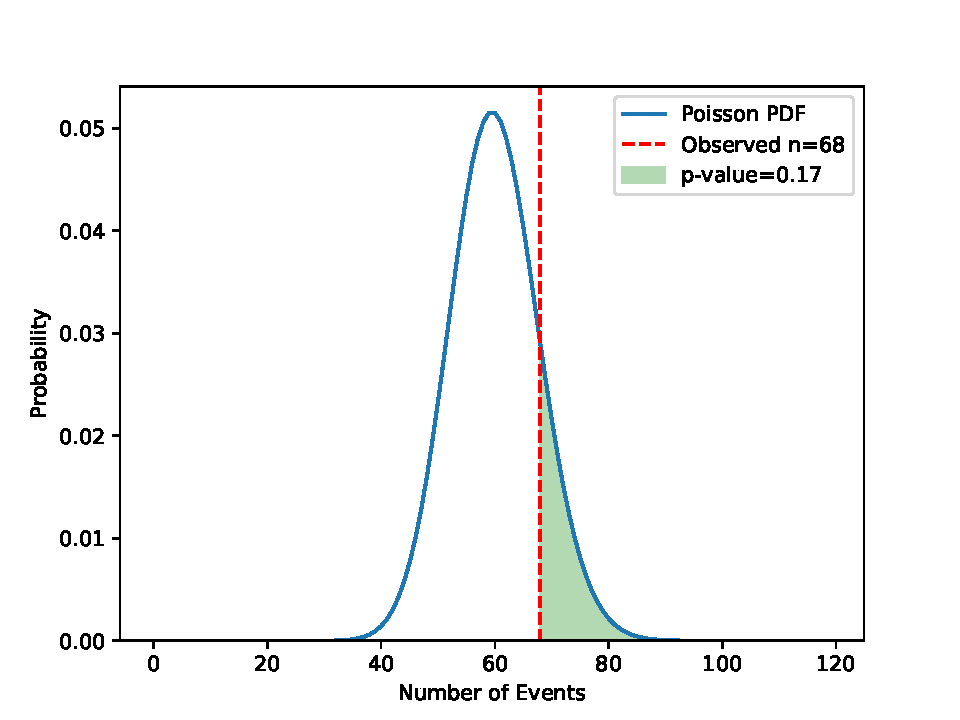
\includegraphics[width=\linewidth,height=\textheight,keepaspectratio]{results/toy_poisson}
            \caption{Toy Poisson PDF}
            \label{fig:poisson_toy_sig:pdf}
        \end{subfigure}
        \begin{subfigure}{0.48\textwidth}
            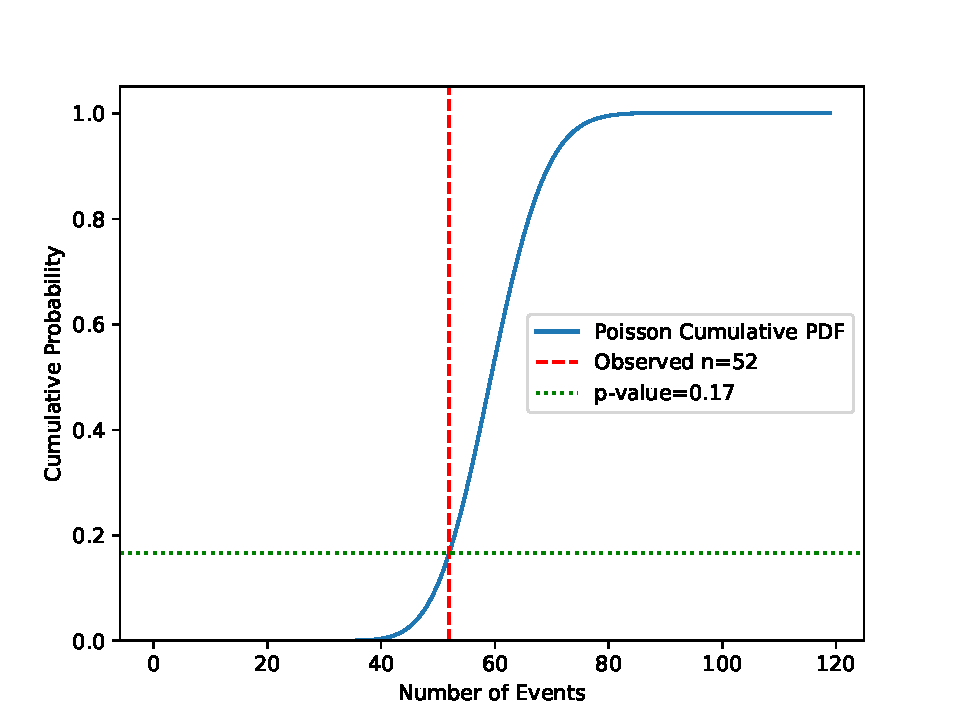
\includegraphics[width=\linewidth,height=\textheight,keepaspectratio]{results/toy_Cpoisson}
            \caption{Toy Poisson Cumulative PDF}
            \label{fig:poisson_toy_sig:Cpdf}
        \end{subfigure}
        \caption{
            A plot of the probability distribution function (PDF)
                and cumulative PDF for a toy Poisson experiment.
        }
    \end{figure}

    \FloatBarrier
    A ``p-test'' is the key tool that will be used throughout the rest of the analysis.
    Its function is to find the probability that, were my hypothesis correct,
        I would obtain data with a value \textit{at least as extreme} as what I measured\footnote{
            There are actually several different variations of a p-test;
            this is specifically a one-sided p-test}.
    So the p-value for an event rate of 68, given an expected average of 60, can be found by taking:
    \begin{equation}
        \textrm{p-value}(n=68) = P(68|60) + P(69|60) + P(70|60) ... P(\infty|60) = \sum\limits_{m=n}^\infty P(m|60)
    \end{equation}
    This is best visualized using the \textit{cumulative} probability distribution function (Fig. \ref{fig:poisson_toy_sig:Cpdf}).
    In this example, the p-value would be 0.17.
    A typical standard for many statistical tests, and the one used in this analysis,
        is to establish a ``Confidence Level'' (CL) in the results of an experiment at a level of 95\%. 
    The confidence level is simply $1-p$, so a CL of 0.95 corresponds to a p-value of less than 0.05.
    Because this toy experiment has a p-value larger than 0.05,
        the conclusion would be that ``the hypothesis was compatible with the data within a CL of 95\%.''
    [Hey Steve, assuming I should even keep my example here, I'm not sure I'm wording this precisely as needed 
        I know these conclusion statements are touchy with their wording;
        should I adjust the toy numbers to make for a better example?]


    % Introduce background
    % Ditch toy, pull out actual Background and Signal (SM) event yields.
    % Should also probably dig up the "sensitivity" metric and show how bad that is here as well.
    % CLs = CLs+b/CLb explained in (Barlow:2019svl pg. 192)
    % The abysmal performance here should justify splitting the event into bins,
    %     in order to identify regions of Mhh that we are more sensitive to.
    % Using multiple bins however, dramatically complicates the statistical analysis.
    % Enter the profile likelihood fit.
    Moving on from the toy example, the hypothesis being tested in this analysis
        involves a background event rate in addition to the signal hypothesis being considered.
    The average number of events expected is then $\nu = S + B$,
        where $S$ and $B$ are the signal and background rate yields respectively.
    The confidence limits in such a situation are handled in different ways from one analysis to another,
        but in this analysis the p-value of the signal alone is given by
    \begin{equation}
        P_S = \frac{P_{S+B}}{1 - P_B}
    \end{equation}
    Where $P_{S+B}$ is the p-value of the hypothesis assuming the signal is present,
        and $P_B$ is the p-value of the background-only hypothesis
        (often called the ``null hypothesis,'' $H_0$)\cite{Barlow:2019svl}.
    The total yields of the data, Background estimate, and SM signal hypothesis are provided in Table \ref{tab:event_yield},
        and their PDF and cumulative PDF can be seen in
        Fig. \ref{fig:poisson_sig:pdf} and \ref{fig:poisson_sig:Cpdf}.

    \begin{table}[tbh]
       \begin{center}
           \caption{Estimated and Observed Event Yields [FIXME: put in the real data once you have it]}
           \label{tab:event_yield}
           \footnotesize
           \begin{tabular}{|l|l|}
           \toprule
               Type  &	Event Yield \\
               \midrule
               Background Estimate  & 7012 \\
               Signal Hypothesis (SM) & 0.36 \\
               %Signal Hypothesis (\kvv=3) & 400 \\
               Observed Data & 7053 \\
           \bottomrule
           \end{tabular}
       \end{center}
    \end{table}

    \begin{figure}
        \centering
        \begin{subfigure}{0.48\textwidth} 
            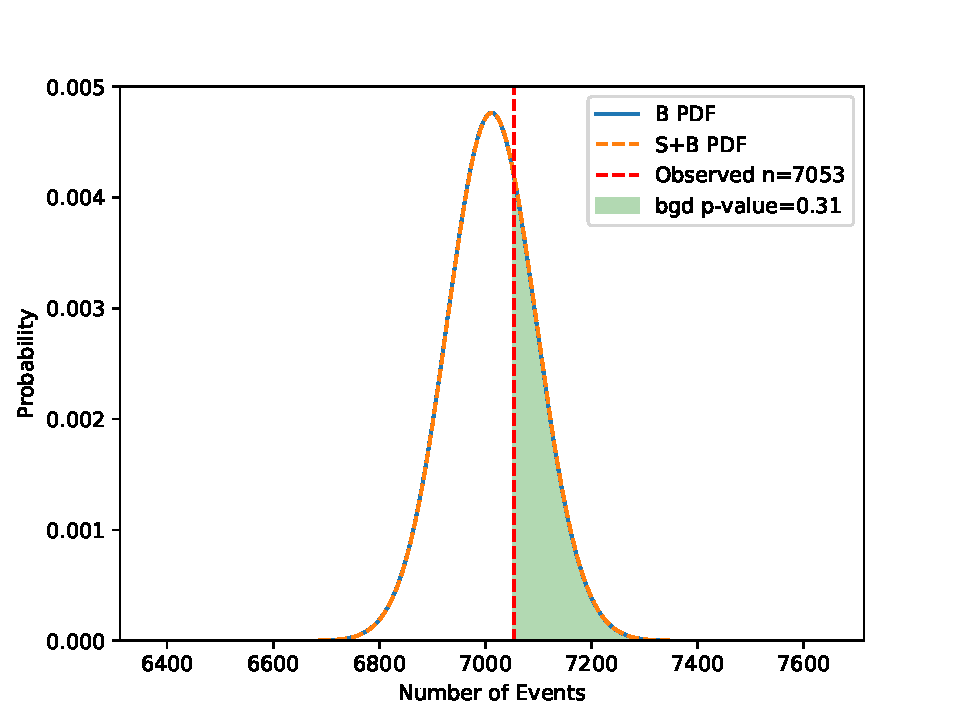
\includegraphics[width=\linewidth,height=\textheight,keepaspectratio]{results/total_yield_poisson}
            \caption{Poisson PDF}
            \label{fig:poisson_sig:pdf}
        \end{subfigure}
        \begin{subfigure}{0.48\textwidth}
            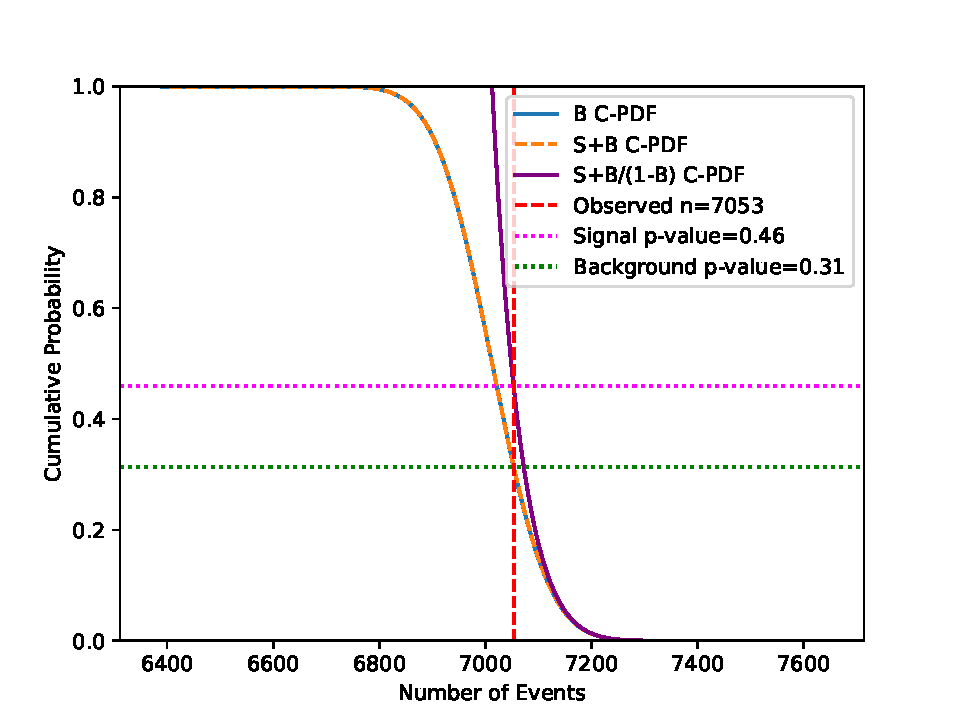
\includegraphics[width=\linewidth,height=\textheight,keepaspectratio]{results/total_yield_Cpoisson}
            \caption{Poisson Cumulative PDF}
            \label{fig:poisson_sig:Cpdf}
        \end{subfigure}
        \caption{
            A plot of the probability distribution function (PDF)
                and cumulative PDF for the estimated background and simulated signal,
                with the observed yield denoted in both.
        }
    \end{figure}

    The p-value of the signal based on the observed yield is 0.46,
        for a CL of 54\%.
    This indicates that the signal is very compatible with the data,
        but by no means indicates proof for the di-Higgs process.
    To understand why, one need only look at the CL on the background-only hypothesis.
    Proof of the di-Higgs process would necessitate an excess of events so significant that
        the null hypothesis must be rejected (typically $P_B < 10^{-7}$, the ``$5\sigma$'' discovery limit).
    Here though, $P_B = 0.31$, which means the null hypothesis is \textit{also} highly compatible with the data,
        and cannot be rejected.

    \begin{figure}
        \centering
        \begin{subfigure}{0.48\textwidth} 
            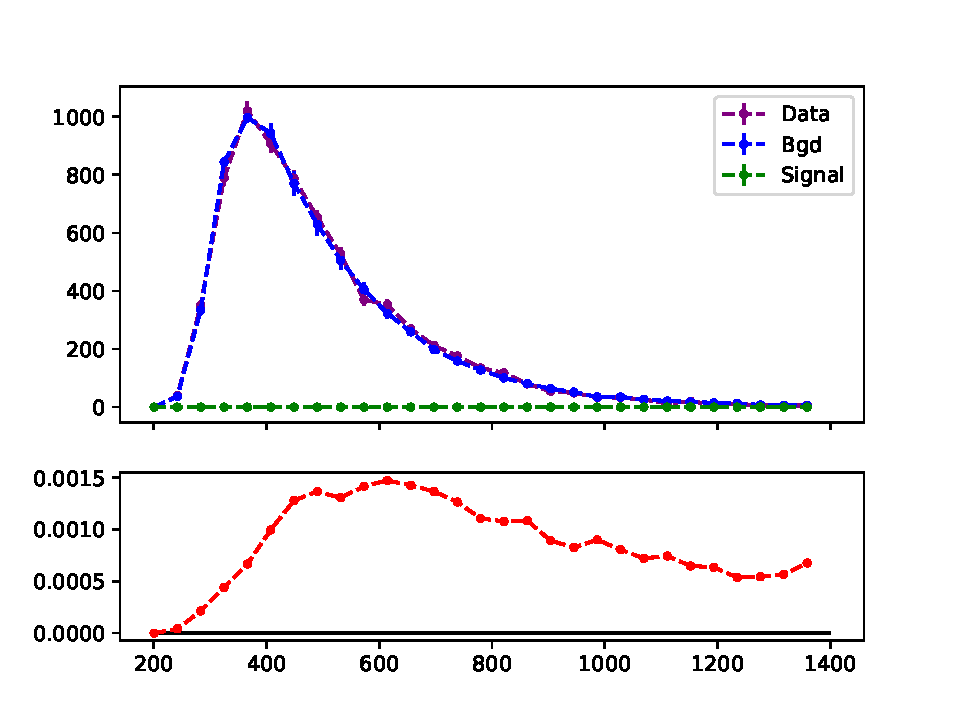
\includegraphics[width=\linewidth,height=\textheight,keepaspectratio]{results/mhh_yield_SM}
            \caption{Event yields with SM Signal [TODO: make this plot better with labels and stuff]}
            \label{fig:mhh_yield:kvv1}
        \end{subfigure}
        \begin{subfigure}{0.48\textwidth}
            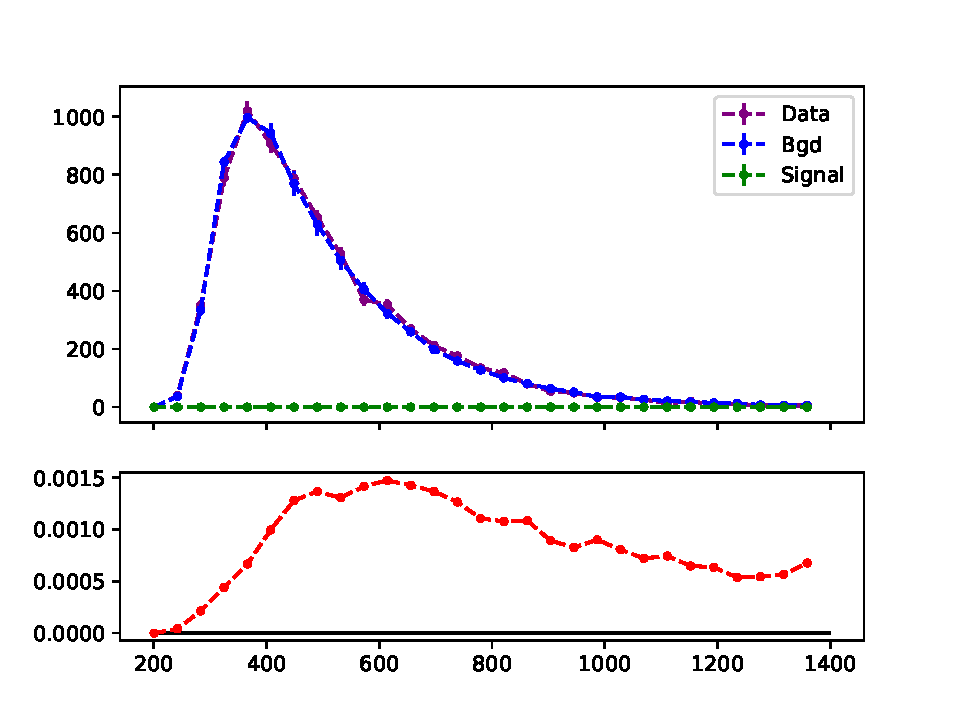
\includegraphics[width=\linewidth,height=\textheight,keepaspectratio]{results/mhh_yield_SM}
            \caption{Event yields with Signal \kvv=3 [TODO: actually grab the kvv=3 distro]}
            \label{fig:mhh_yield:kvv3}
        \end{subfigure}
        \caption{
            The event yields of the data, background, and signal binned by their \mhh distribution.
            The bottom plot displays the ``sensitivity'' ($Z_s=\frac{S}{\sqrt{S+B}}$)
                of the analysis to a particular \mhh bin.
            A sensitivity value of $\approx 2$ is usually necessary to achieve a CL around 95\%.
            [Hey Steve do I need to explain sensitivity in detail? Also do I have this right?]
        }
    \end{figure}


    The issue of course, is that the signal is utterly dwarfed by the quantity of background events.
    A method of circumventing this scale issue
        is to break the event count up across a number of different
        bins and categories dependent on kinematic observables of the events.
    The signal and background events are expected to have their events distributed differently across such observables.
    Thus, even though there are vastly more background events overall,
        it is entirely possible for there to exist a region in the observable space
        in which there are a comparable number of signal events.
    In this analysis, the primary observable variable is the di-Higgs invariant mass, \mhh.
    Ultimately, the final test of the hypothesis will still be to create a cumulative PDF distribution,
        obtain the p-value of the cumulative PDF for the observed data, and use that to derive a CL for the signal.
    With multiple bins (as well as categories and uncertainties) however,
        the derivation of the cumulative PDF becomes much more complex.
    The following section will describe precisely how all these aspects of the analysis are combined together,
        producing a much more powerful statistical analysis.


\FloatBarrier
% Discuss sources of error, assumptions, categorization, concept of mu values;
% basically all the complicated stuff the limit framework is doing
% Make the final goal to be establishing a p-value via the cumulative PDF distro,
%   as was done for the simple coin toss example (to bring things full circle)
\section{VBF HH 4b Limit-Setting Framework}
    
    %What is a test statistic and why do we need it?
    The statistical technique used here to obtain a cumulative PDF
        is based on the use of a ``test statistic'' derived through a \textit{profile likelihood fit}.
    Test statistics come in many forms, but the one used here is the \qtil test statistic.
    \qtil is technically defined in a single equation,
        but that equation involves so many parameters that it is worth breaking it down into steps.

    % Introduce mu*S+B format.
    % Discuss formula for L specifically in this analysis
    %    (emphasis on explaining the bits in parentheses):

    %    L = product[ for each category (2: eta hi and lo) 
    %        product[for each bin: poissons]
    %        * product[ nuissance params (4 for bgd shape error, 1 for norm error) ] 
    %    ]
    %    
    The first step to deriving \qtil is to slightly redefine the expectation value for the number of events 
        with a scaling factor $\mu$ applied to the signal yield.
    $\mu$ is referred to as the ``Parameter of Interest'' (PoI),
        and allows the yield of the signal process to be adjusted to some ideal value that best fits the data.
    As well, since there are now multiple bins $i$ (each with their own expectation values)
        the new definition of the expectation value is
    \begin{equation}
        \nu_i(\mu) = \mu S_i + B_i
    \end{equation}
    Instead of a probability distribution function, now a ``likelihood'' function $L$ will be used,
        which is the joint probability of the observed data $n$ in each of the bins
        (which are in turn all Poisson distributed with expectation value $\nu_i$)
    \begin{equation}
        L(n,\mu) = \prod \limits_{i=1}^{N} P(n_i | \nu_i)
            = \prod \limits_{i=1}^{N} \frac{ (\mu S_i + B_i)^{n_i} e^{\mu S_i + B_i} }{n_i!}
    \end{equation}
    Where $i$ runs over all the $N$ bins.
    Note that unlike a PDF, the sum of all outcomes from the likelihood function will \textit{not} sum to unity,
        and so the likelihood function does not constitute a probability distribution function\cite{cousins2020likelihood}.

    % Discuss uncertainties and categories
    Uncertainties present in the background estimate add another layer of complexity to the likelihood function,
        because uncertain parameters must be fit as well as the parameter of interest.
    The expectation value is further adjusted to be $\nu_i(\mu, \Theta) = \mu S + \Theta B$,
        where $\Theta$ is a product of five scaling values 
    \begin{equation}
        \Theta = \prod \limits_{a=0}^{4}  \theta^a
    \end{equation}
    These scaling values, called ``nuisance parameters,''
        correspond to the four shape uncertainties $\sigma_i^a, a\in{1,2,3,4}$
        and one normalization uncertainty $\sigma^0$ ($\sigma^0$ does not vary by bin),
        which were described in Section \ref{sec:nn_training}
        [TODO: you need to go back and describe these uncertainties better now that you understand them].
    Here the background uncertainty is modeled as a Gaussian with expectation value $\theta^a B_i$ and standard deviation $\sigma_i^a$.
    Extending the likelihood function with the nuisance parameters produces
    \begin{equation} \begin{split}
        L(n,\mu,\Theta) &= \prod \limits_{i=1}^{N} P_{\textrm{poiss}}(n_i | \nu_i) 
             \prod \limits_{a=0}^{4} P_{\textrm{gauss}}(n_i | \nu_i, \sigma_i^a) 
        \\&= \prod \limits_{i=1}^{N} \frac{ (\mu S_i + \Theta B_i)^{n_i} e^{\mu S_i + \Theta B_i} }{n_i!} \times
            \prod \limits_{a=0}^4 \frac{1}{\sigma_i^a \sqrt{2\pi}} e^{
                -\frac{1}{2}\left(\frac{n_i- (\mu S_i + \Theta B_i)}{\sigma_i^a}\right)^2
            }
    \end{split} \end{equation}

    Finally, in order to increase sensitivity further, events are split into two different categories
        based on whether the \deta separation between the reconstructed Higgs Bosons is greater or less than 1.5.
    The full likelihood function is then a product over the two categories
    \begin{equation}
        L(n,\mu,\Theta) = \prod \limits_{j=1}^{2}
             \prod \limits_{i=1}^{N} P_{\textrm{poiss}}(n_{ij} | \nu_{ij}) 
             \prod \limits_{a=0}^{4} P_{\textrm{gauss}}(n_{ij} | \nu_{ij}, \sigma_{i}^a) 
    \end{equation}

    % Discuss nuissance parameter fitting
    There is only one parameter of interest ($\mu$), but there are now six parameters $L$ is a function of.
    To address this without over-fitting to the data, a maximized fit is performed across the nuisance parameters.
    Such a fit eliminates their presence from the likelihood function, but it should be noted that it does so at a cost.
    The nuisance parameter fit significantly extends the final cumulative PDF, reducing the overall confidence intervals.
    To perform this fit, the value of $\mu$ is fixed to the desired scale (for now $\mu=1$),
        and then $L(n,\mu,\Theta)$ is maximized over the various values of the $\theta^a$.
    The nuisance parameter values are then fixed to this maximal value $\hat{\hat\theta}^a$, such that
    \begin{equation}
        \prod \limits_{a=0}^{4} \frac{\partial}{\partial \theta^a} L(n,\mu,\Theta) |_{\Theta=\hat{\hat\Theta}} = 0
    \end{equation}
    Resulting in a fitted $L = L(n,\mu,\hat{\hat\Theta})$.
    [TODO: I still don't know how the stat errors get factored into all this...
        are they treated the same way as the nuissance params,
        or are they somehow intrinsic to the poisson distribution?
    Stat error for poisson is just sqrt(expectation),
        so maybe the stat error is automatic?
    Or is there some deeply unpleasant error propogation going on under the pyhf hood?]
        
    %lambda = L(mu, theta vary-opt) / L(mu-opt, theta-opt);
    As a final fitting step, the likelihood $L$ is normalized to a fully maximized value $\hat L$,
        to create a quantity $\lambda = L / \hat L$.
    $\hat L$ is formed in a similar manner to $L$, but whereas $L$ has a fixed value for $\mu$,
        $\hat L$ allows $\mu$ to also be a free parameter.
    It is then maximized with regard to both $\mu$ and the nuisance parameters such that
    \begin{equation}
        \prod \limits_{a=0}^{4} \frac{\partial}{\partial \theta^a} \frac{\partial}{\partial \mu} L(n,\mu,\Theta) |_{\Theta=\hat \Theta} |_{\mu=\hat \mu} = 0
    \end{equation}
    A test statistic $t$ can now be constructed with $\lambda$, as
    \begin{equation}
        t = -2 \ln{\lambda} = -2 \ln{\frac{L(\mu, \hat {\hat \Theta})}{L(\hat \mu, \hat \Theta)}}
    \end{equation}
    It is worth briefly reviewing what this formula and its pieces mean before moving onto the last step.
    The likelihood $L$ is just the joint probability that every bin of the observed data would have the values they do,
        based on the modeled expectation values.
    Due to the large number of bins, $L$ will always be an extremely small number between 0 and 1.
    By construction, $\hat L$ will always be a joint probability at least as large as $L$, though still between 0 and 1.
    Their ratio $\lambda$ represents how close $L$ is to being maximally likely for the given set of observed data and models.
    $\lambda$ can at most be equal to 1, indicating that $L$ is nearly equal to $\hat L$,
        which in turn indicates that the model fits the observed data as well as it can for any given value of $\mu$.
    In turn, a value near 0 indicates that the observed data is exceedingly unlikely to have come from the model with the given $\mu$,
        compared to the much more likely model based on the optimal value of $\mu$.
    The test statistic $t$ then has a simple interpretation:
        values of $t$ close to 0 indicate high likelihood,
        and the higher the value of $t$ (up to infinity) the more unlikely it is that the model is compatible with the data.

    %q~ = t with edge cases;
    At last, the desired test statistic \qtil can be derived, as a piece-wise variation on $t$\cite{asymptotic_formulae_for_likelihood}:
    \begin{equation}
        \qtil = \begin{cases}
            -2 \ln{\frac{L(\mu, \hat {\hat \Theta})}{L(0, \hat \Theta(\mu=0))}} & \hat \mu < 0,\\
            -2 \ln{\frac{L(\mu, \hat {\hat \Theta})}{L(\hat \mu, \hat \Theta)}} & 0 \leq \hat \mu \leq \mu,\\
            0 & \mu < \hat \mu 
        \end{cases}
    \end{equation}
    The middle condition is simply $t$, with the top and bottom edge cases being the defining traits of \qtil.
    \qtil in particular is used for this analysis because of these piece-wise conditions,
        which enforce the fact that $\mu$ should never be negative (the signal cannot remove events from the background),
        and that this analysis is only interested in establishing a lower-bound
        [TODO: might need to think about this some more to be sure you know what you're saying here].

    %Single mu vs q~ PDF constructed from monte-carlo distros
    %C-PDF showing where mu-model resides for Psb, Pb, and finally Ps=Psb/(1-Pb)
    %In practice, the q~ CPDF distros are estimated using an asymptotic approximation method\cite{asymptotic_formulae_for_likelihood}.
    %(because the MC method is way too slow)
    Even with the test statistic \qtil available, its use may not be immediately obvious.
    Recall that the goal is to produce a cumulative probability distribution function,
        which can be compared against to obtain a p-value.
    In order to obtain a distribution, it must be created using Monte-Carlo techniques.
    A large number of simulated distributions can be generated,
        sampled from the modeled signal and background Poisson distributions.
    For each of these simulated ``observations'' the test statistic \qtil can be derived.
    The result is a collection of \qtil values, which together comprise a distribution.
    A cumulative probability distribution can be constructed with this distribution,
        by simply taking the fraction of simulated observations which fall below some value of the observed \qtil.
    Figures \ref{fig:qtil:pdf} and \ref{fig:qtil:Cpdf} demonstrate how this is done,
        as well as where the SM signal model falls with a $\mu$ value of 1.

    \begin{figure}
        \centering
        \begin{subfigure}{0.48\textwidth} 
            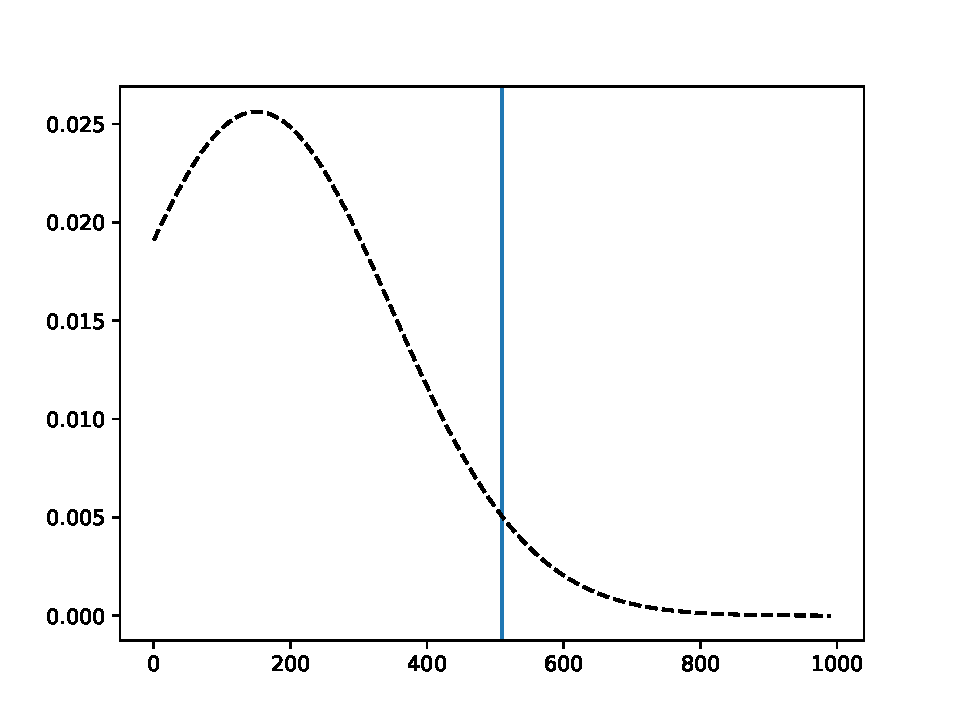
\includegraphics[width=\linewidth,height=\textheight,keepaspectratio]{results/mu_pdf}
            \caption{Values of \qtil for Simulated Distributions}
            \label{fig:qtil:pdf}
        \end{subfigure}
        \begin{subfigure}{0.48\textwidth}
            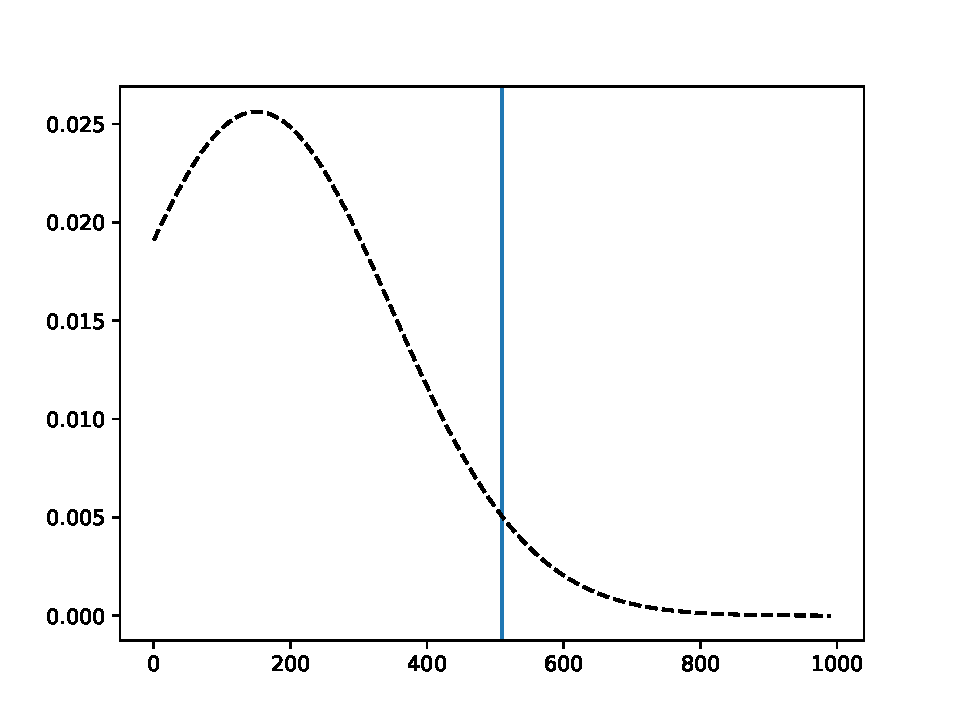
\includegraphics[width=\linewidth,height=\textheight,keepaspectratio]{results/mu_pdf}
            \caption{Cumulative PDF of \qtil Test Statistic}
            \label{fig:qtil:Cpdf}
        \end{subfigure}
        \caption{
            [TODO: replace the placeholders with the real thing.]
            [Steve, so these will be by far the most involved plots here,
                because I'm trying to generate them by reverse engineering the entire limit framework and pyhf.
            If I can finish them, it's a nice proof to myself that I understand how everything is actually done.
            But I may not have enough time to finish this,
                in which case I'll probably just scrap these figures and the references to them.]
            Plots of the values and cumulative PDF based on \qtil,
                with the \qtil value of the observed data highlighted.
            Note the ``error bands'' which provide extended regions of higher confidence.
            These are produced via the formula [TODO: how do I still not know how these are made?!].
        }
    \end{figure}

    I would like to note that while I have performed the explicit simulation of the MC distributions for the sake of these figures,
        in practice the MC approach is far too slow.
    What is often done instead, and what this analysis in particular does (via the Pyhf python framework),
        is to use an asymptotic approximation to the \qtil cumulative distribution function.
    The derivation of this approximation is well beyond the scope of this thesis,
        but is documented extensively by Cowan\cite{asymptotic_formulae_for_likelihood}.
    \qtil itself still needs to be calculated for the observed data,
        but the asymptotic approximation allows for rapid and accurate calculation of its p-value.
    Now that I finally have a robust mechanism for calculating the p-value of the di-Higgs signal hypothesis,
        the only step remaining is to use it.

\FloatBarrier
% Finally, I need to reveal what our final results actually are, and what they mean.
% This will mostly just be plots of mu values, limit values, and my 2D exclusion plots.
% I can discuss the shapes and stuff here, as well as talk about any mismatches between expected and observed results.
% Be ready to just put in filler results, since we probably won't have unblinded by the time I get here.
\section{Final Interpretation}

    [Hey steve, for this first edit round, don't worry about the formatting of any of the plots in this section.
    They all need to be replaced when we unblind, and we've been updating their format a lot. (these are pretty old)]
    [FIXME: literally all the plots and numbers and conclusions here need to be updated once we unblind]
    All limits quoted in this analysis are to a CL of 95\%.
    The CL of the SM signal hypothesis with a $\mu$ scale of 1,
        even with the extensive profile likelihood fit technique, is still only 50\% [FIME].
    No meaningful conclusion can be drawn from such a small signal.
    However, looking at the \kvv=3 signal model at a $\mu$ scale of 1 provides a CL of $\approx 99\%$,
        which indicates that a value of \kvv=3 is incompatible with data, and so can be excluded.
    This result suggests a much more useful way of performing these tests.
    For each signal hypothesis, a series of increasing values of $\mu$ can be tested against the observed data,
        each with their own CL value.
    A series of such tests can be seen in Fig. \ref{fig:mu_CL_vals}.

    \begin{figure}
        \centering
        \begin{subfigure}{0.48\textwidth} 
            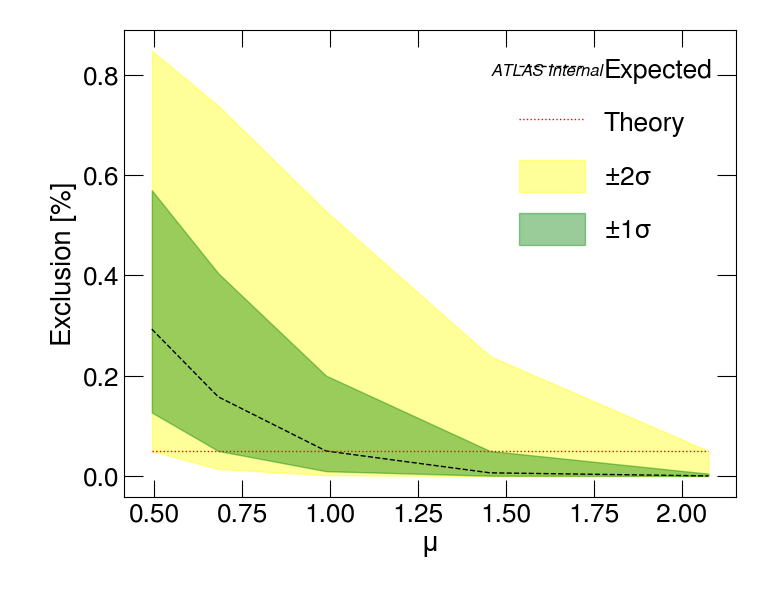
\includegraphics[width=\linewidth,height=\textheight,keepaspectratio]{results/brazilplot_full_3D_scan_NEO2021_samps_vbf_pd_161718_kl_1-00_k2v_0-00_k1v_1-00}
            \caption{Values of \qtil for Simulated Distributions}
            \label{fig:mu_CL_k2v0}
        \end{subfigure}
        \begin{subfigure}{0.48\textwidth} 
            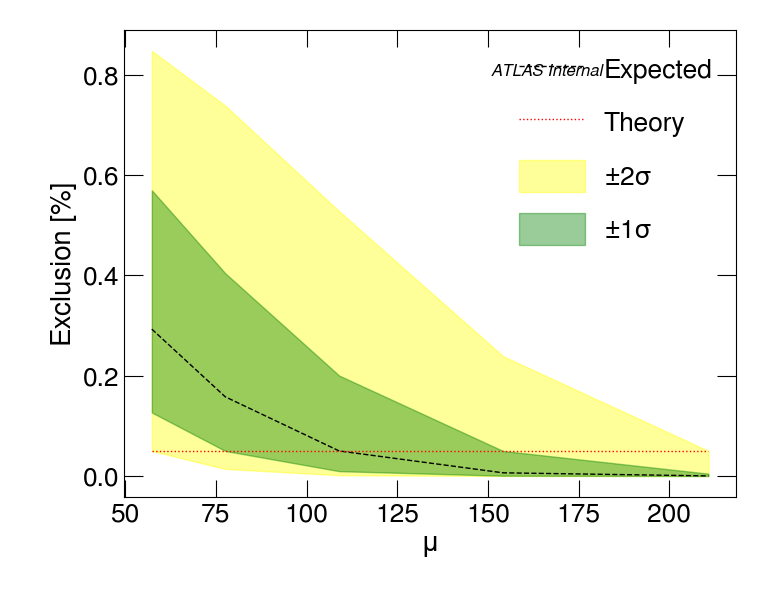
\includegraphics[width=\linewidth,height=\textheight,keepaspectratio]{results/brazilplot_full_3D_scan_NEO2021_samps_vbf_pd_161718_kl_1-00_k2v_1-00_k1v_1-00}
            \caption{Values of \qtil for Simulated Distributions}
            \label{fig:mu_CL_k2v1}
        \end{subfigure} \\
        \begin{subfigure}{0.48\textwidth}
            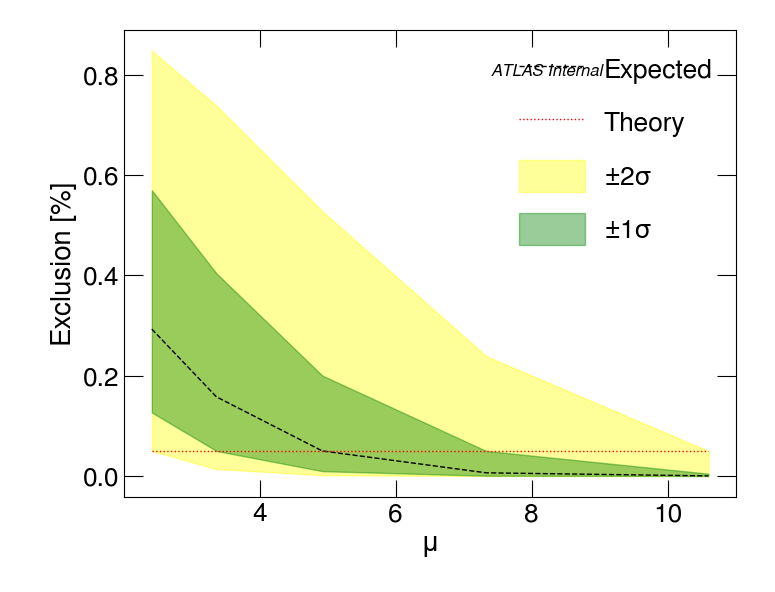
\includegraphics[width=\linewidth,height=\textheight,keepaspectratio]{results/brazilplot_full_3D_scan_NEO2021_samps_vbf_pd_161718_kl_1-00_k2v_1-50_k1v_1-00}
            \caption{Cumulative PDF of \qtil Test Statistic}
            \label{fig:mu_CL_k2v1.5}
        \end{subfigure}
        \begin{subfigure}{0.48\textwidth}
            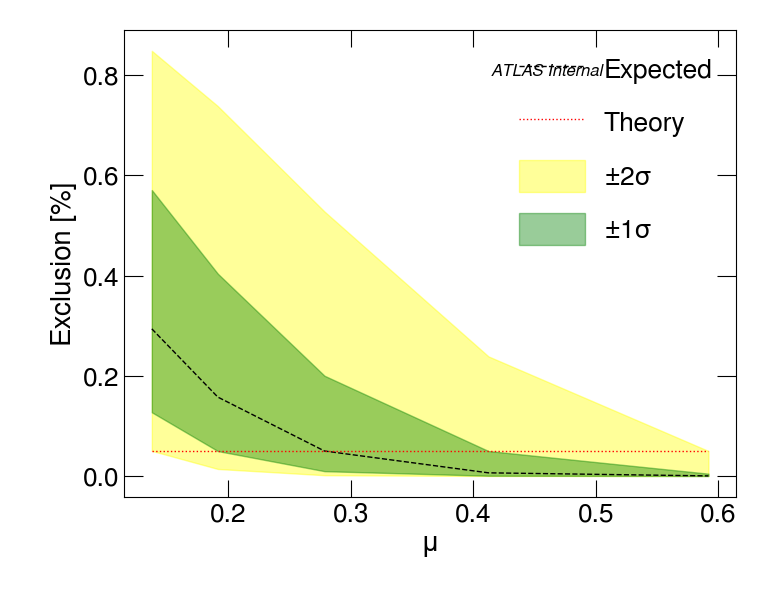
\includegraphics[width=\linewidth,height=\textheight,keepaspectratio]{results/brazilplot_full_3D_scan_NEO2021_samps_vbf_pd_161718_kl_1-00_k2v_3-00_k1v_1-00}
            \caption{Cumulative PDF of \qtil Test Statistic}
            \label{fig:mu_CL_k2v3}
        \end{subfigure}
        \caption{
            [Wow the labels on these plots are super wrong. Pretty sure y is supposed to be the p-value,
                and the red line is the 0.05 mark. I think these are fixed in the updated plots?]
        }\label{fig:mu_CL_vals}
    \end{figure}

    \FloatBarrier
    The critical value for each of the plots in Fig. \ref{fig:mu_CL_vals} is the 95\% CL $\mu$.
    A more general plot can be created from this by showing the CL=95\% $\mu$
        exclusion value as a function of the coupling value $\kvv$.
    Utilizing the signal model linear combination equation from Section \ref{sec:signal_combination},
        the signal hypothesis for any value of \kvv can be tested, producing Fig. \ref{fig:kvv_SM_scan}.

    \begin{figure}
        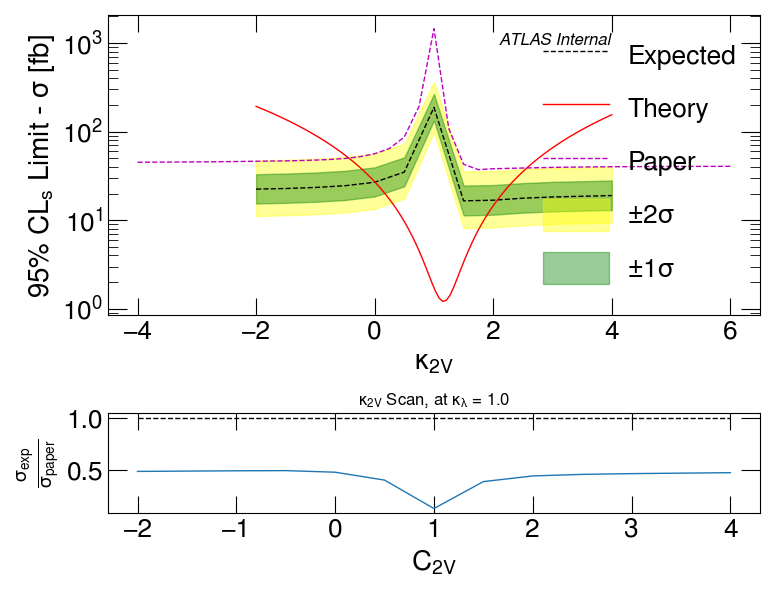
\includegraphics[width=\linewidth,height=\textheight,keepaspectratio]{results/k2v_scan_full_3D_scan_NEO2021_samps_vbf_pd_161718_kl_1-0_xsec.png}
        \caption{DiHiggs signal \kvv exclusion plot.
            The red line indicates the theoretical cross-section of the di-Higgs interaction as a function of \kvv.
            The dashed line is formed as the product of the theoretical cross-section value
                and the 95\% CL value of $\mu$ for that \kvv signal}
        \label{fig:kvv_SM_scan}
    \end{figure}

    Figure \ref{fig:kvv_SM_scan} is arguably the single most significant result presented in this thesis,
        as it indicates that \kvv=0 can be excluded with a CL of 95\% [To Steve: look I can hope alright].
    This in turn provides strong evidence for the existence of the \HHVV interaction process.
    Yet, there is still more to discuss.

    The signal combination formula is able to produce a signal hypothesis with multiple coupling values adjusted at once,
        and so a wide range of \kvv scan plots can be produced, as seen in Fig. \ref{fig:kvv_multi_kl}

    \begin{figure}
        \centering
        \begin{subfigure}{0.48\textwidth} 
            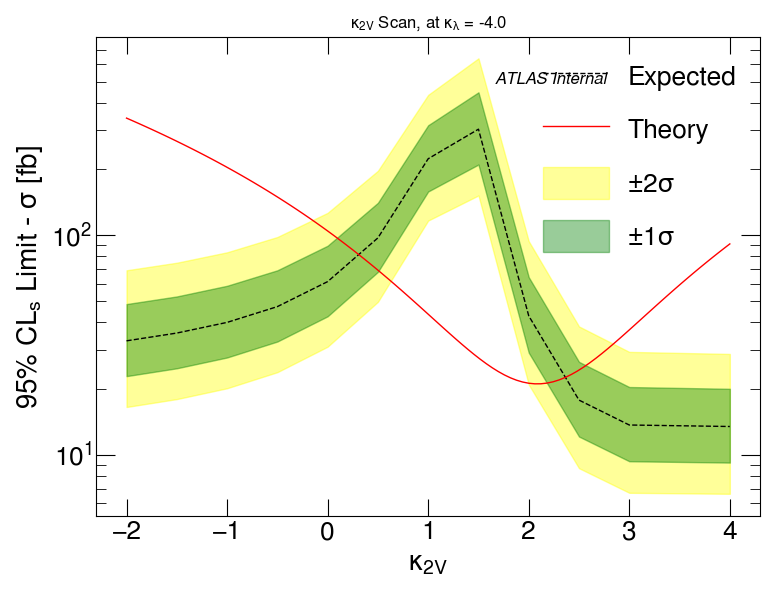
\includegraphics[width=\linewidth,height=\textheight,keepaspectratio]{results/k2v_scan_full_3D_scan_NEO2021_samps_vbf_pd_161718_kl_-4-0_xsec.png}
            \caption{\kvv Exclusion, \kl=-4}
            \label{fig:kvv_scan_kl0}
        \end{subfigure}
        \begin{subfigure}{0.48\textwidth} 
            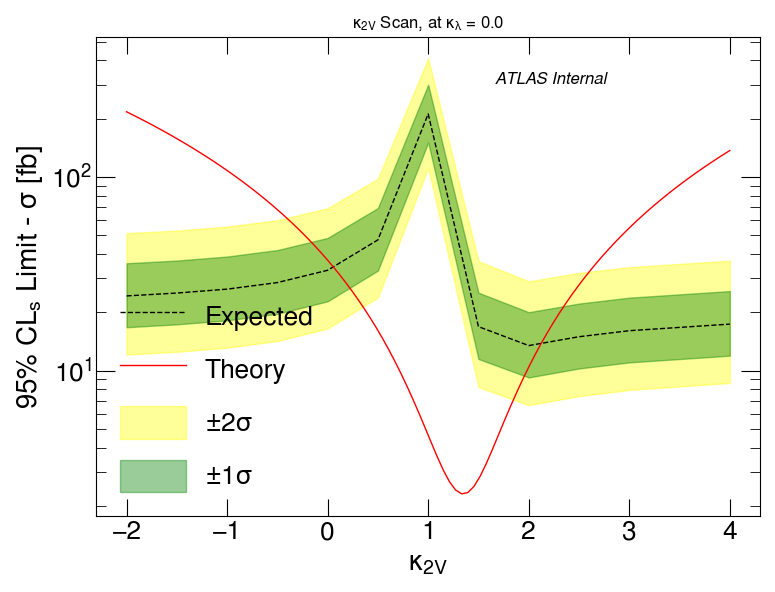
\includegraphics[width=\linewidth,height=\textheight,keepaspectratio]{results/k2v_scan_full_3D_scan_NEO2021_samps_vbf_pd_161718_kl_0-0_xsec.png}
            \caption{\kvv Exclusion, \kl=0}
            \label{fig:kvv_scan_kl1}
        \end{subfigure} \\
        \begin{subfigure}{0.48\textwidth}
            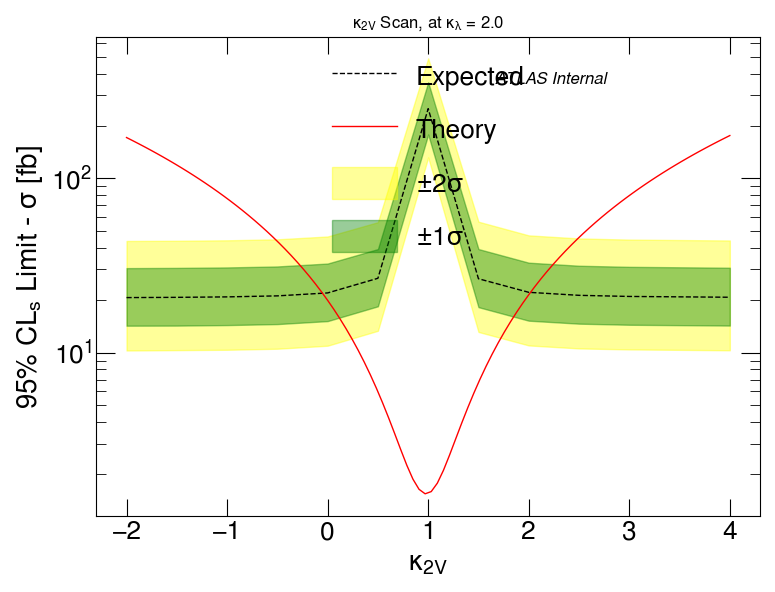
\includegraphics[width=\linewidth,height=\textheight,keepaspectratio]{results/k2v_scan_full_3D_scan_NEO2021_samps_vbf_pd_161718_kl_2-0_xsec.png}
            \caption{\kvv Exclusion, \kl=2}
            \label{fig:kvv_scan_kl2}
        \end{subfigure}
        \begin{subfigure}{0.48\textwidth}
            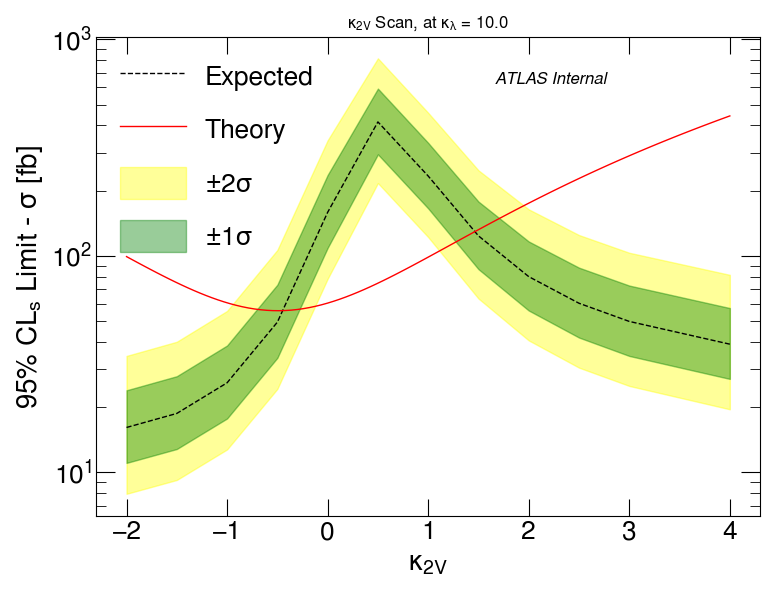
\includegraphics[width=\linewidth,height=\textheight,keepaspectratio]{results/k2v_scan_full_3D_scan_NEO2021_samps_vbf_pd_161718_kl_10-0_xsec.png}
            \caption{\kvv Exclusion, \kl=10}
            \label{fig:kvv_scan_kl10}
        \end{subfigure}
        \caption{
            A collection of \kvv exclusion scan plots, with the \kl coupling set to alternate values.
        }\label{fig:kvv_multi_kl}
    \end{figure}

    \FloatBarrier
    This abundance of parameter space can be collapsed by taking special note only of
        the individual points at which the theoretical cross-section and observed 95\% CL cross-section intersect,
        as these points indicate where the regions of exclusion lie (Fig. \ref{fig:kvv_kl_2Dscan}).

    \begin{figure}
        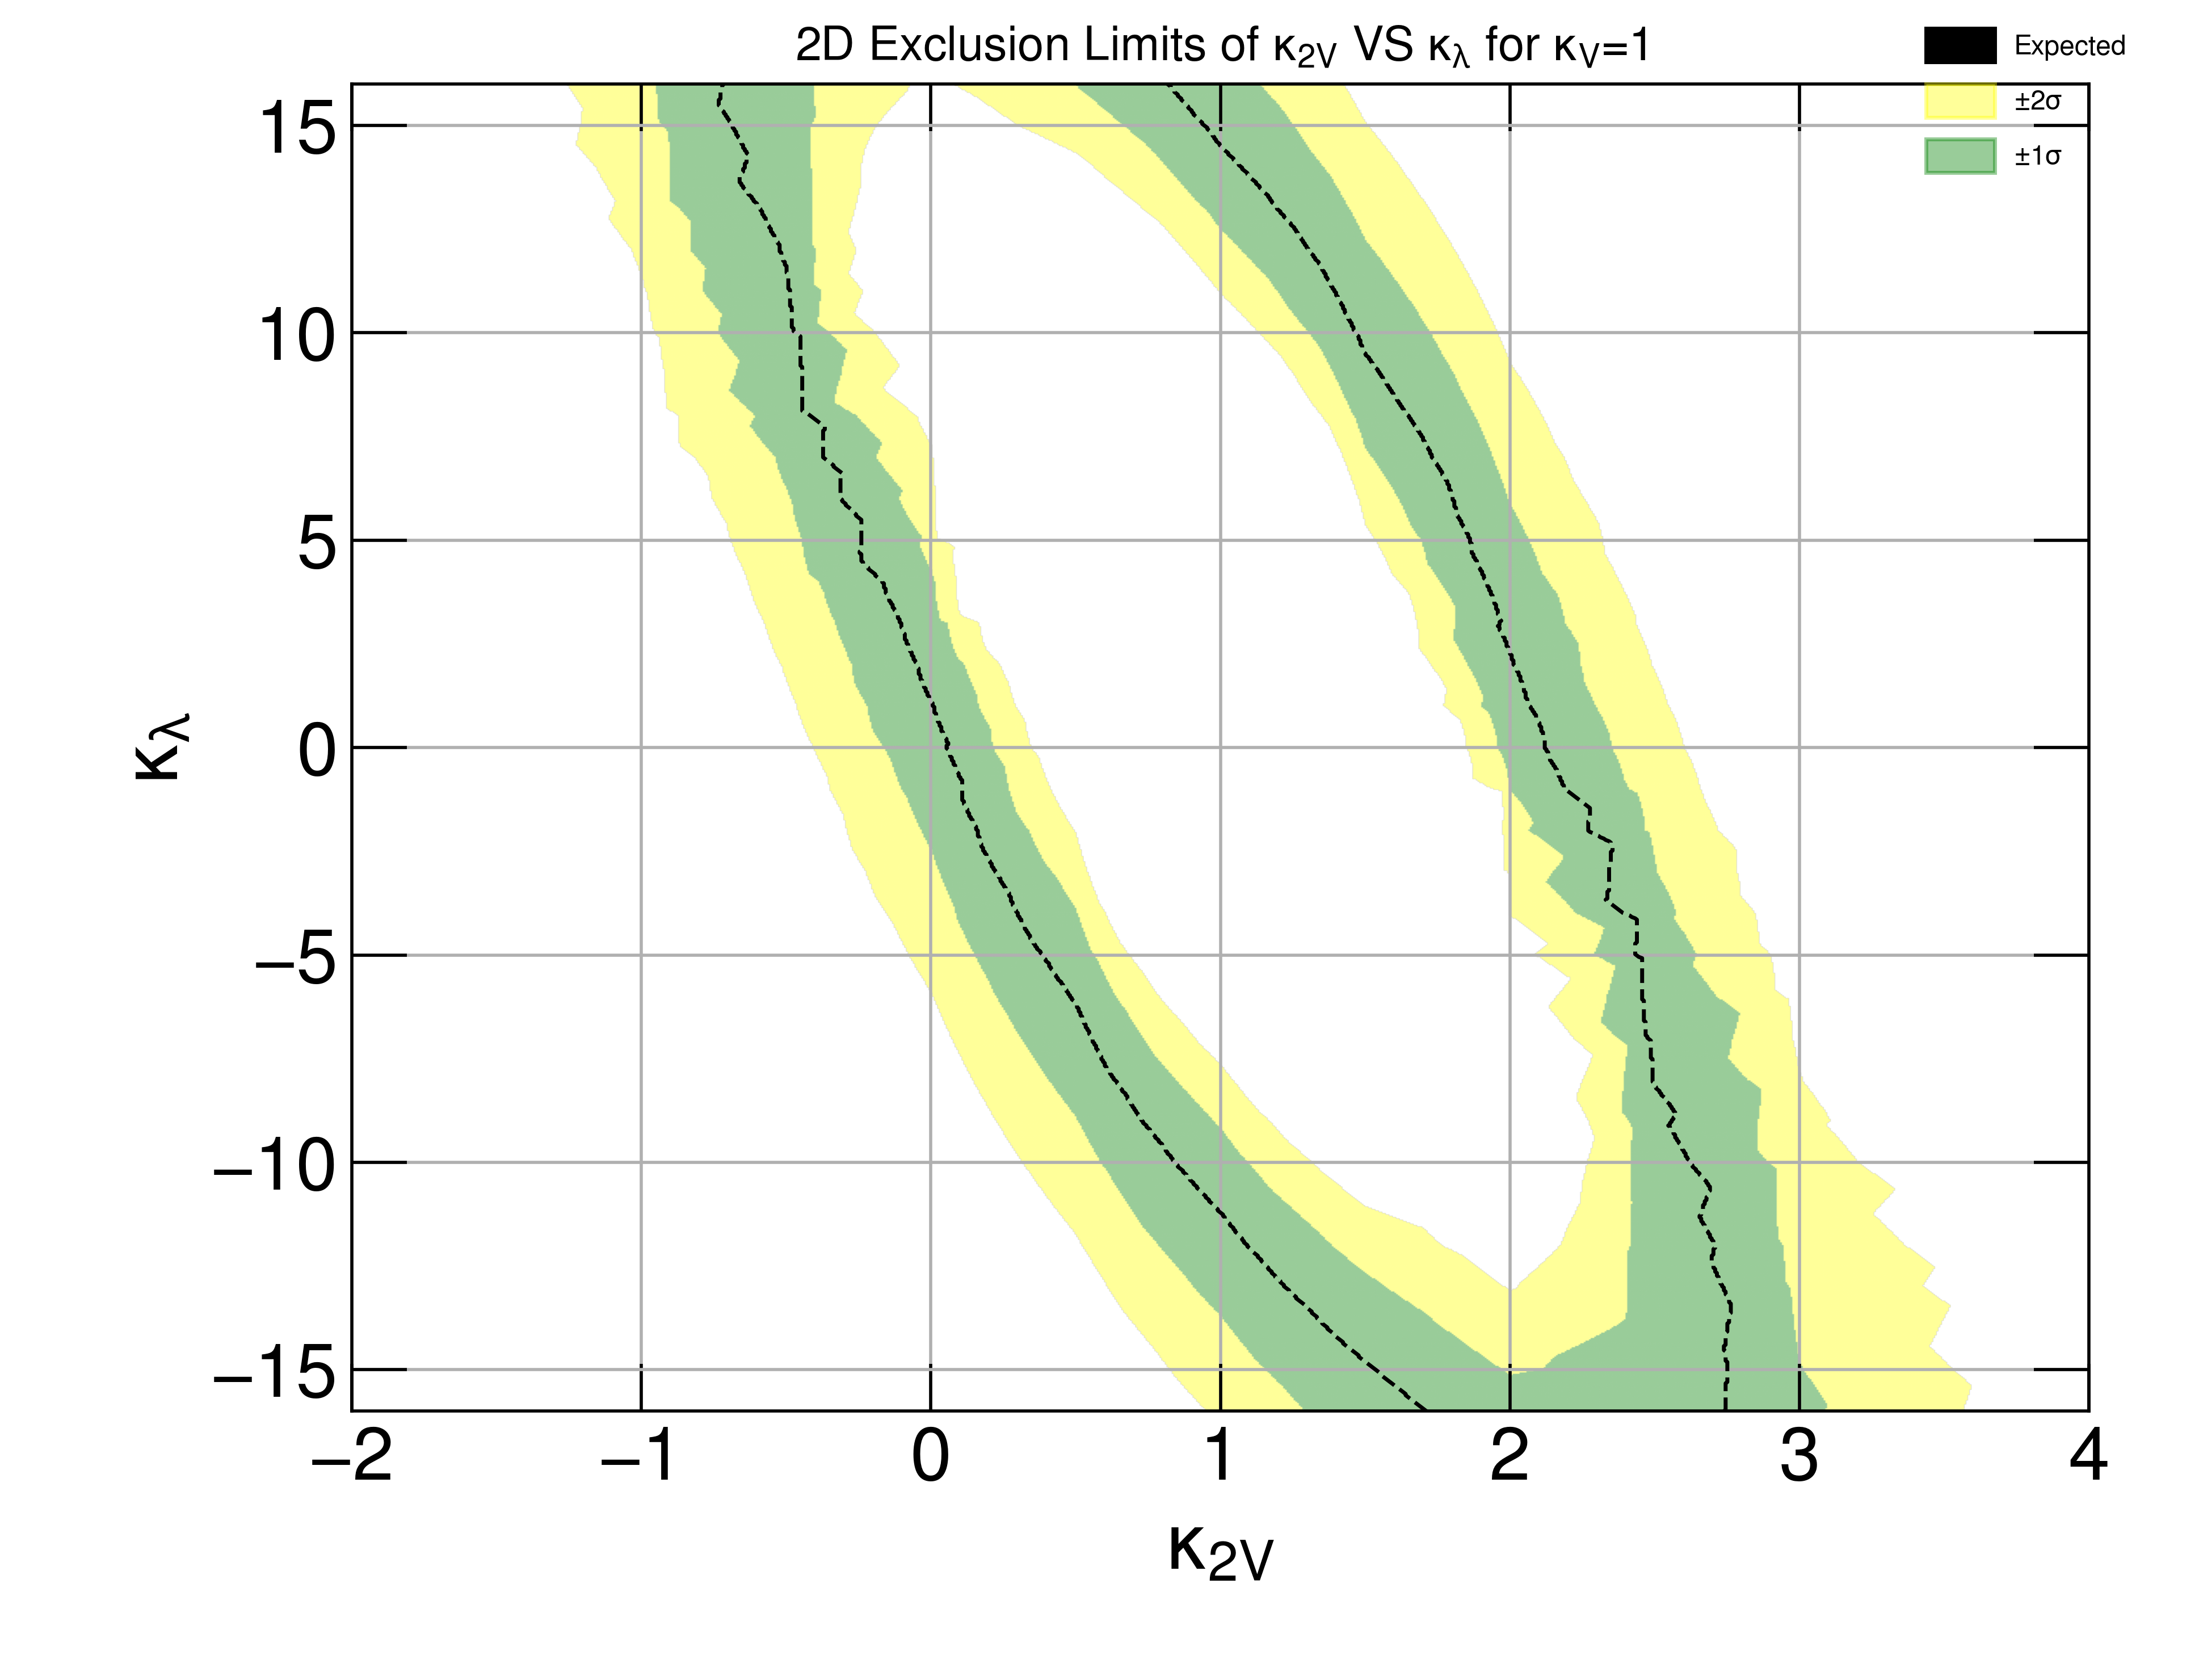
\includegraphics[width=\linewidth,height=\textheight,keepaspectratio]{results/2D_scan_full_3D_scan_NEO2021_samps_vbf_pd_161718_k1v1_exclusion}
        \caption{Two-dimensional \kvv/\kl exclusion plot, for \kv=1.
            Signal hypothesis model corresponding to couplings that lie
                \textit{outside} the ellipsoidal region are incompatible with the observed data to a CL of 95\%,
                and thus can be excluded.
            }
        \label{fig:kvv_kl_2Dscan}
    \end{figure}

    Finally, by utilizing the full dimensionality afforded by the 6-term signal combination equation,
        such scan plots can be produced across multiple slices of \kv.
    \kv is already highly constrained, and Fig. \ref{fig:kvv_kl_multislice}
        reveals that within the established bounds on \kv,
        the constraints on \kl and \kvv differ by very little.

    \begin{figure}
        \centering
        \begin{subfigure}{0.48\textwidth} 
            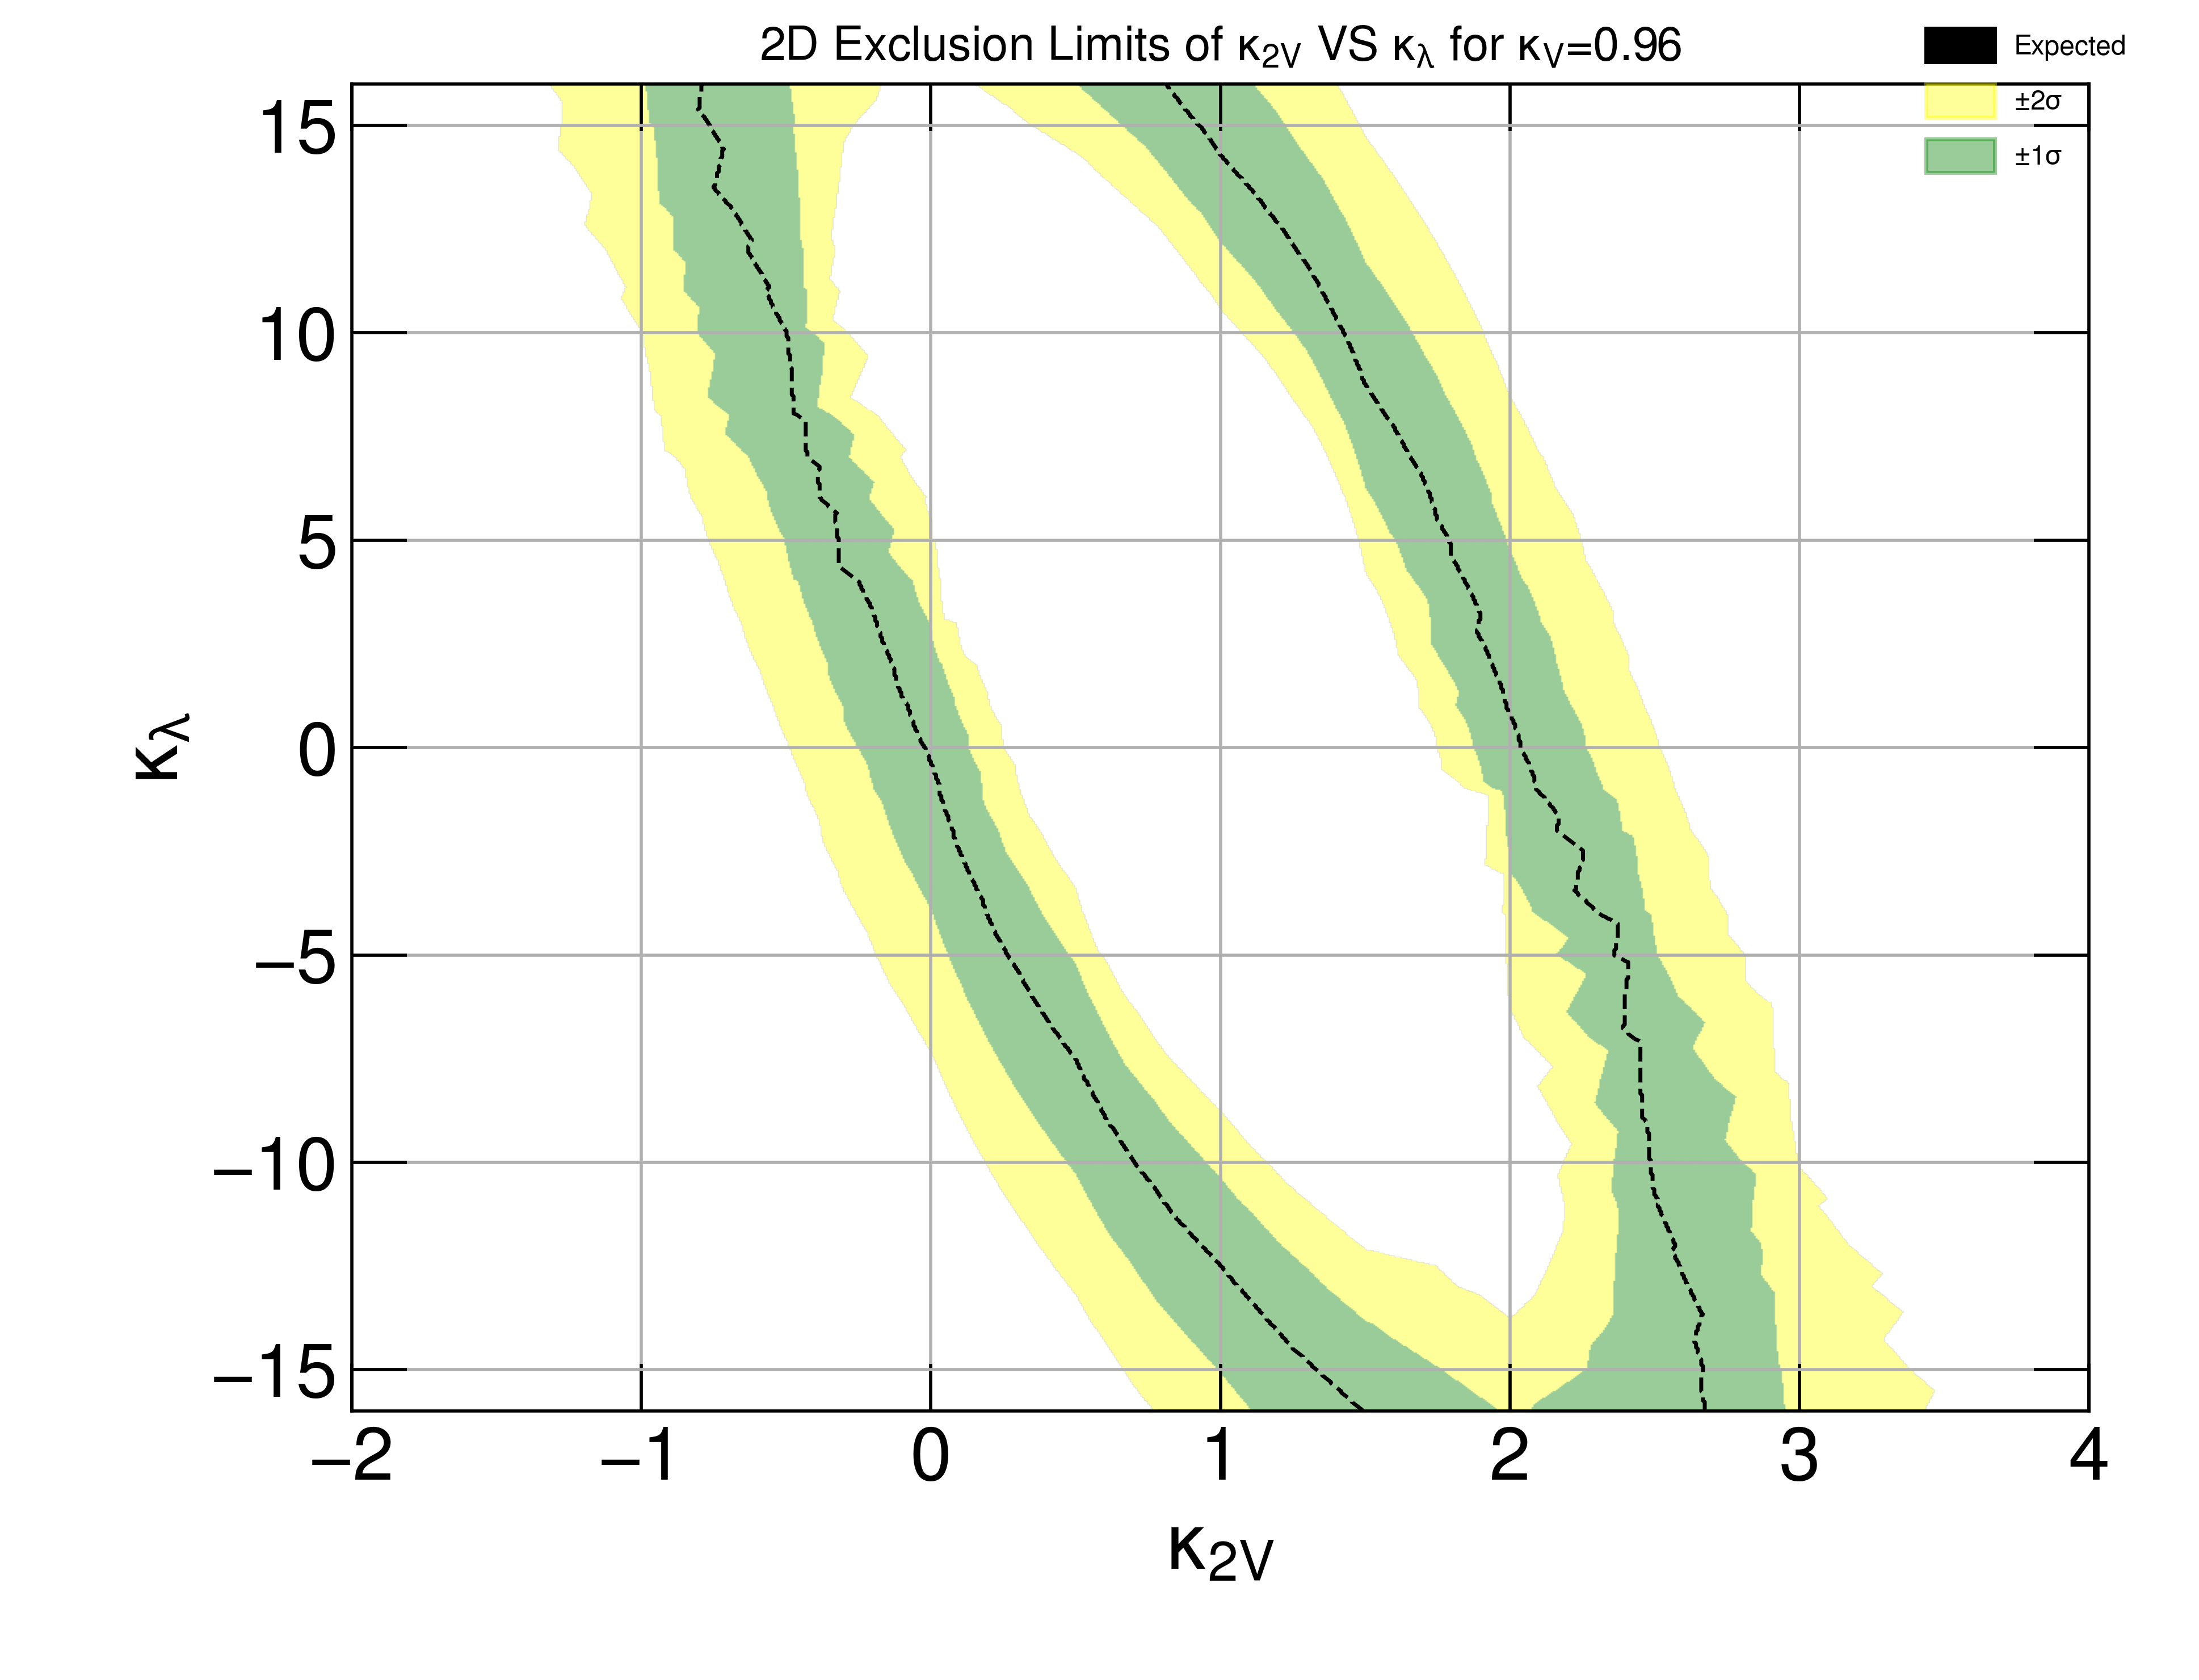
\includegraphics[width=\linewidth,height=\textheight,keepaspectratio]{results/2D_scan_full_3D_scan_NEO2021_samps_vbf_pd_161718_k1v0-96_exclusion}
            \caption{\kvv/\kl Exclusion, \kv=0.96}
            \label{fig:kvv_kl_2Dscan_kv0.96}
        \end{subfigure}
        \begin{subfigure}{0.48\textwidth} 
            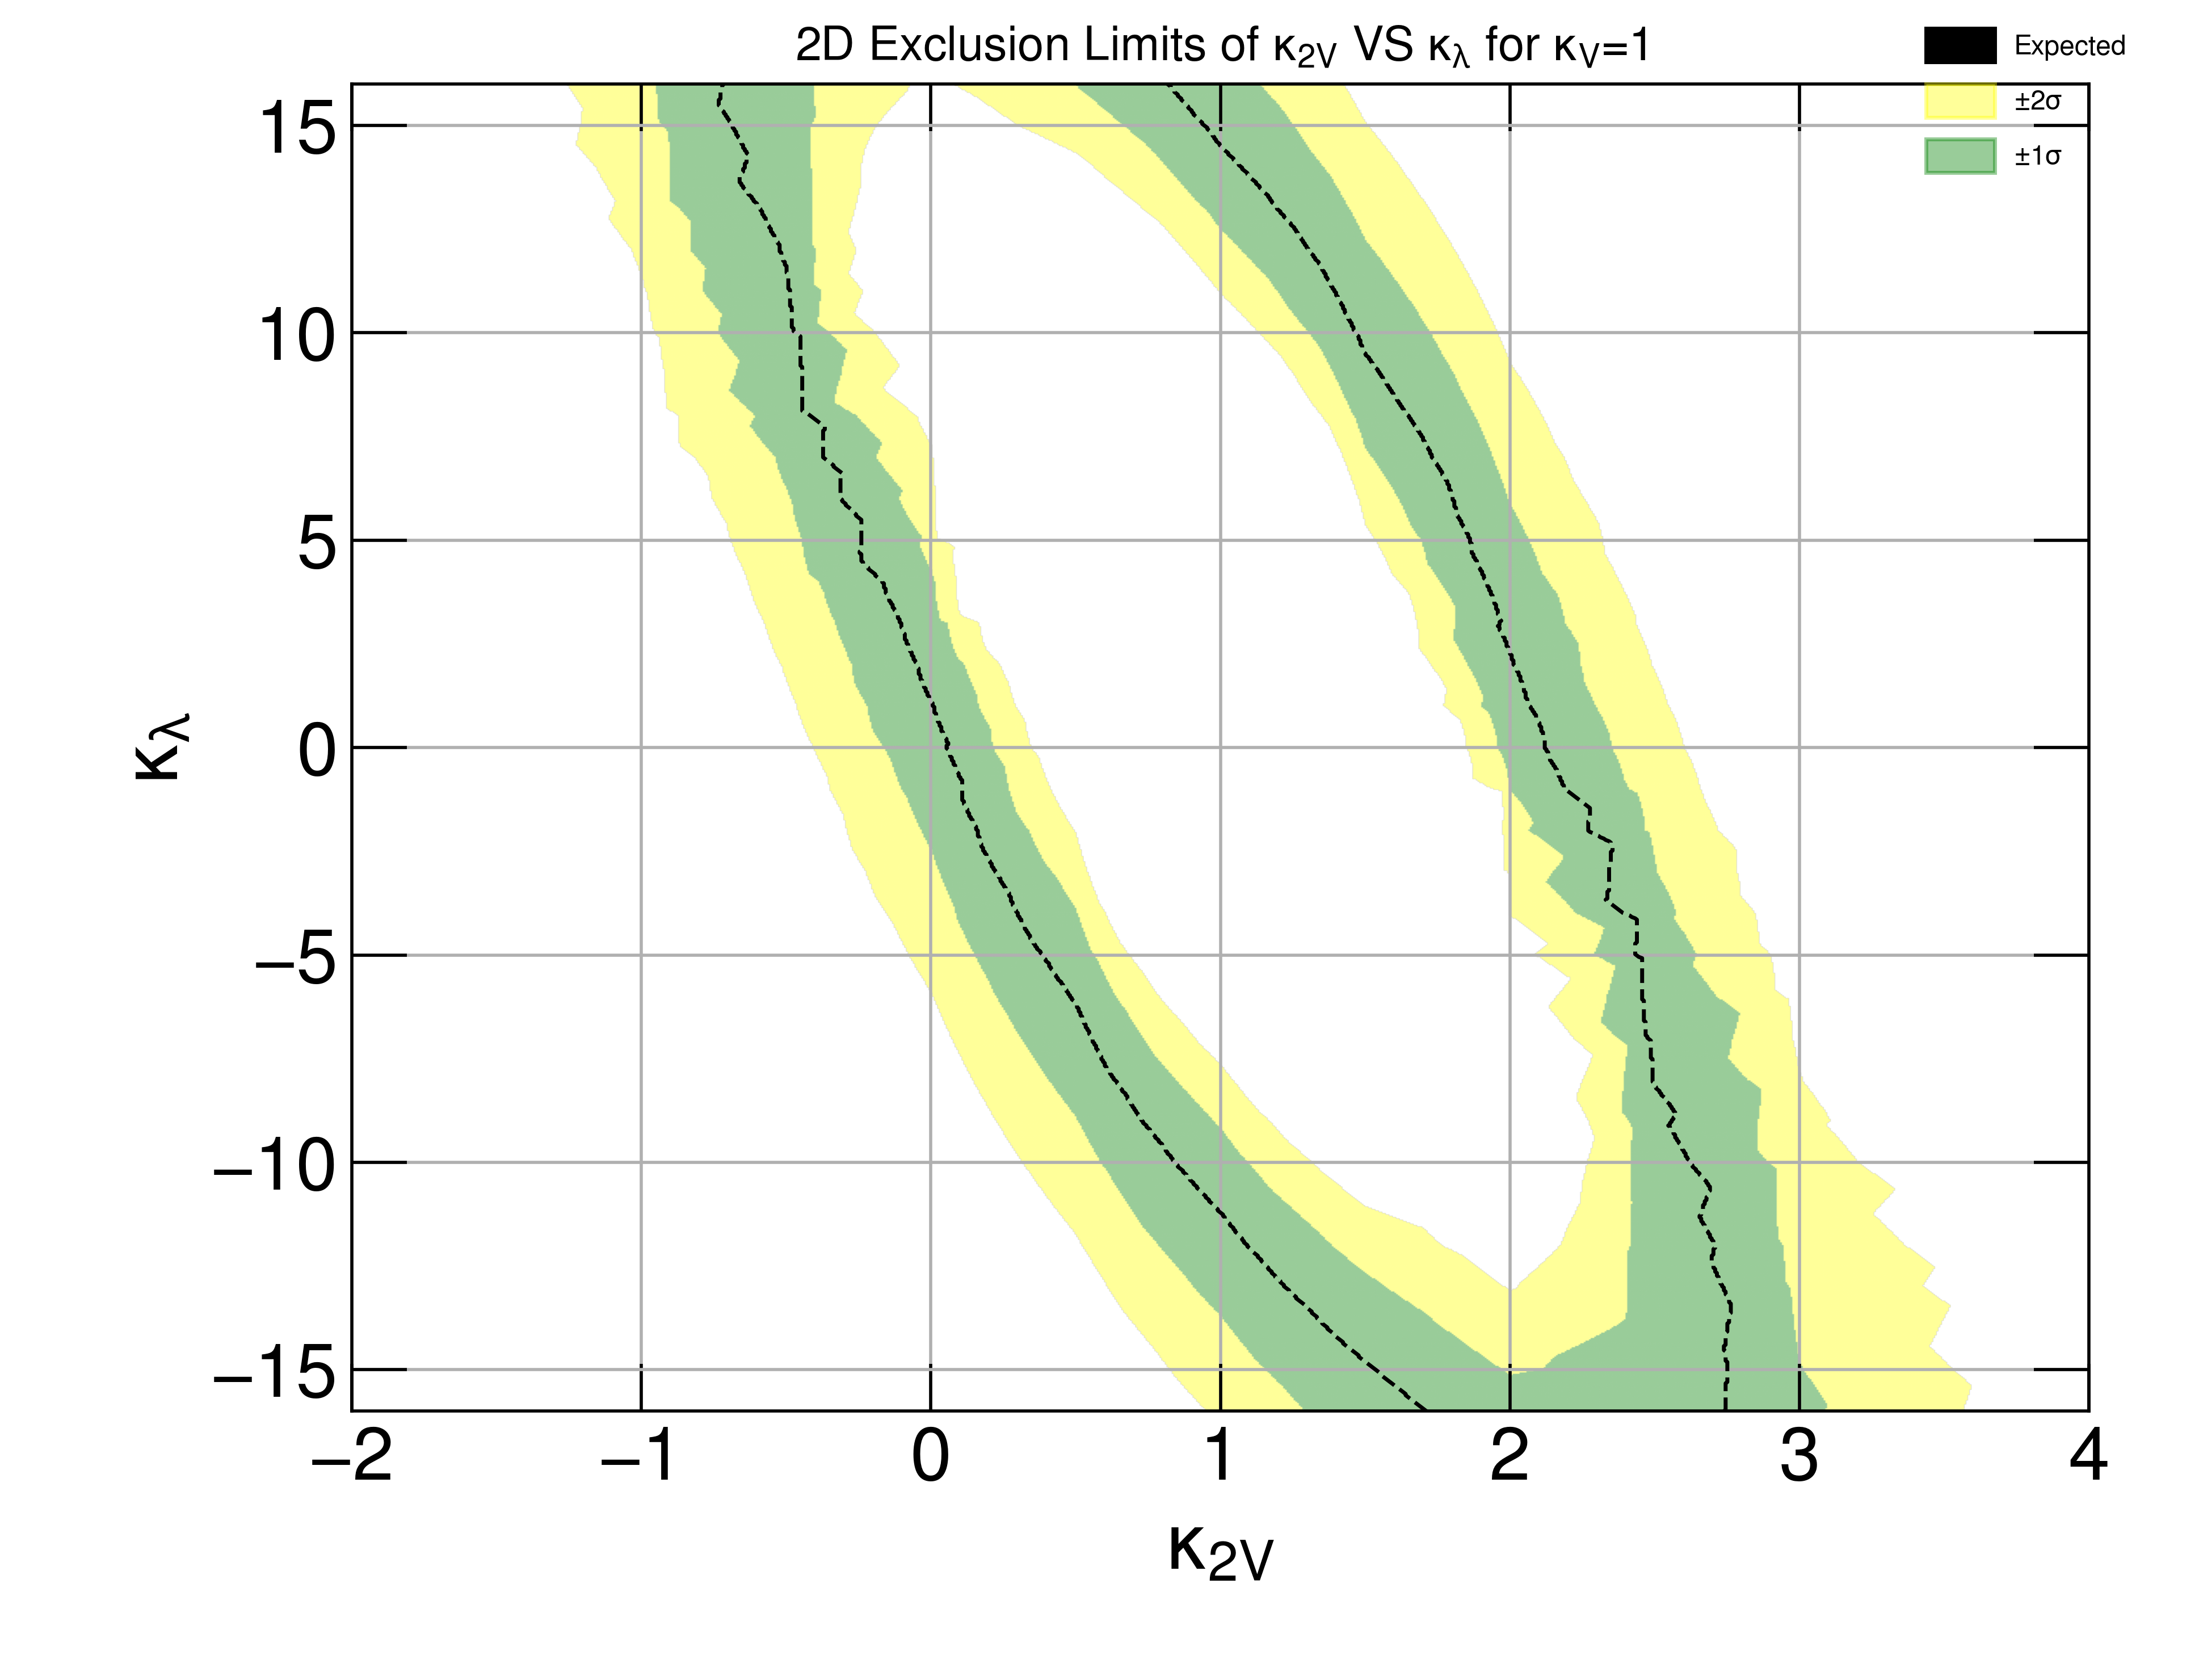
\includegraphics[width=\linewidth,height=\textheight,keepaspectratio]{results/2D_scan_full_3D_scan_NEO2021_samps_vbf_pd_161718_k1v1_exclusion}
            \caption{\kvv/\kl Exclusion, \kv=1.00}
            \label{fig:kvv_kl_2Dscan_kv1}
        \end{subfigure} \\
        \begin{subfigure}{0.48\textwidth}
            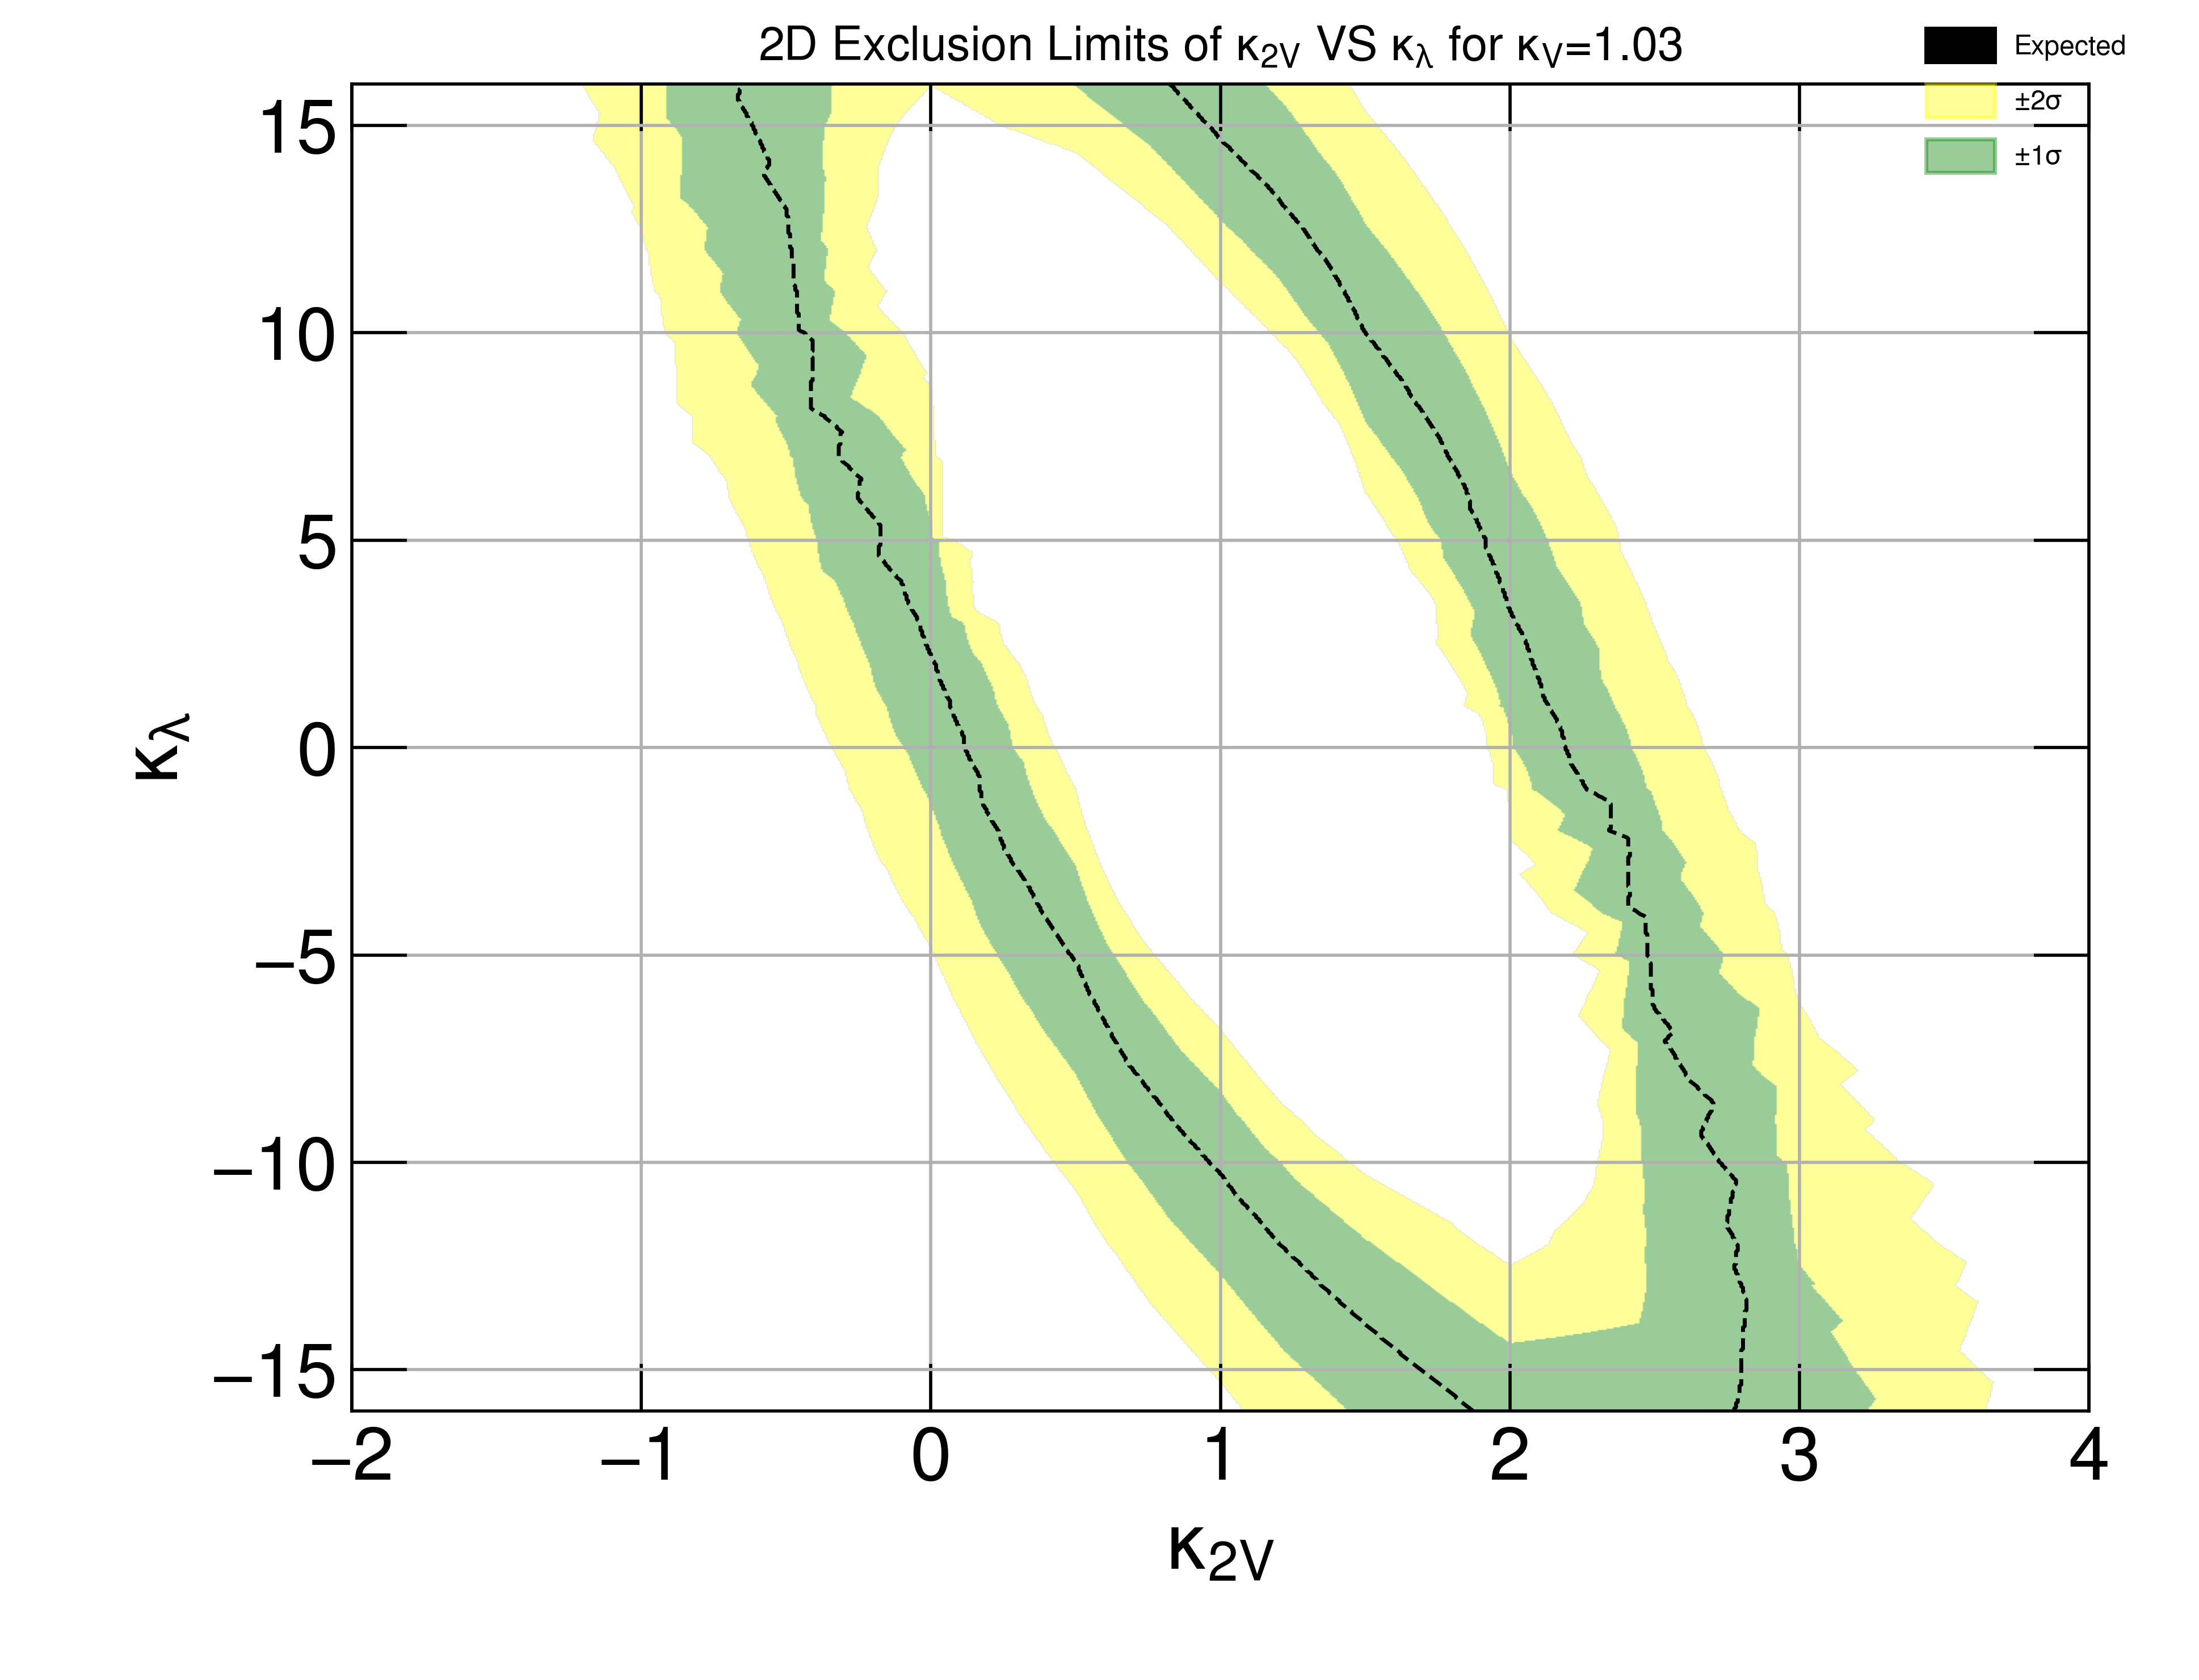
\includegraphics[width=\linewidth,height=\textheight,keepaspectratio]{results/2D_scan_full_3D_scan_NEO2021_samps_vbf_pd_161718_k1v1-03_exclusion}
            \caption{\kvv/\kl Exclusion, \kv=1.03}
            \label{fig:kvv_kl_2Dscan_kv1.03}
        \end{subfigure}
        \begin{subfigure}{0.48\textwidth}
            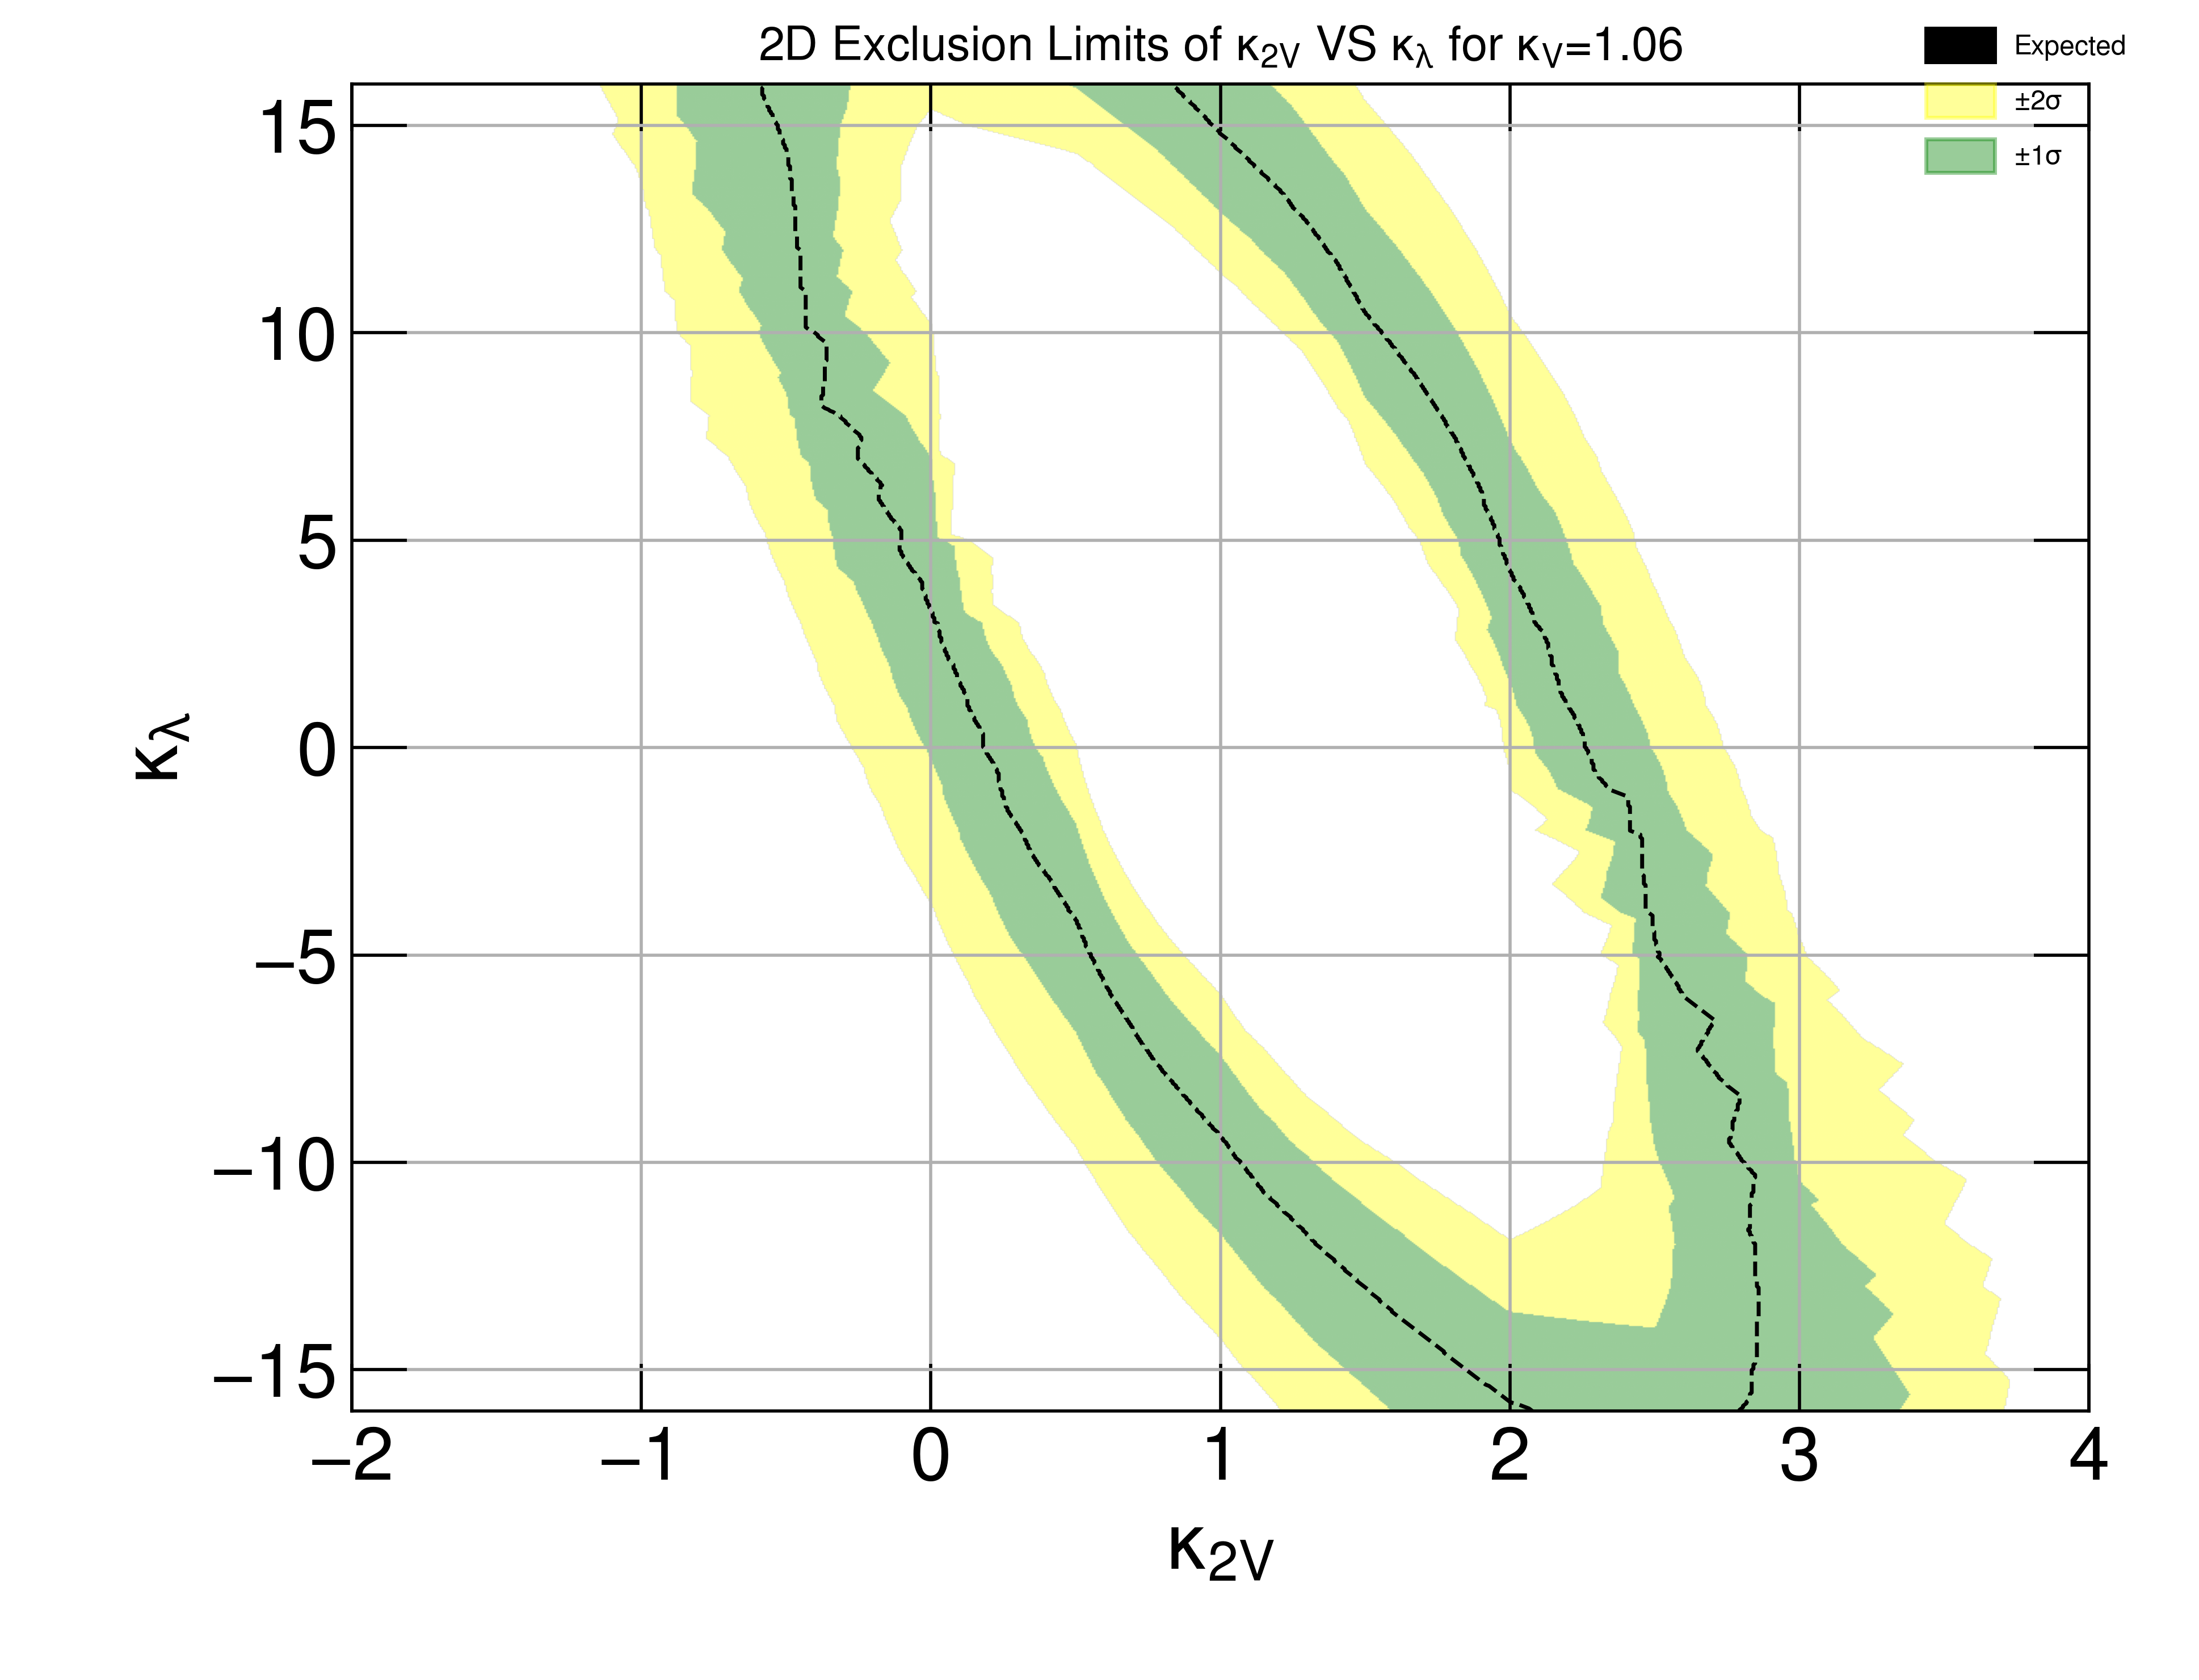
\includegraphics[width=\linewidth,height=\textheight,keepaspectratio]{results/2D_scan_full_3D_scan_NEO2021_samps_vbf_pd_161718_k1v1-06_exclusion}
            \caption{\kvv/\kl Exclusion, \kv=1.06}
            \label{fig:kvv_kl_2Dscan_kv1.06}
        \end{subfigure}
        \caption{Two-dimensional \kvv/\kl exclusion plot, for multiple values of \kv.
            Recall that \kv has been measured as $1.05 \pm 0.04$,
                hence the heavy restriction in its range here.
            Within this range, the \kvv/\kl limits do deviate slightly from their \kv=1 values,
                but not by a dramatic amount.
        }\label{fig:kvv_kl_multislice}
    \end{figure}
